\hypertarget{sec:sota}{%
\chapter{State of the Art}\label{sec:sota}}

The topic of web migration is located in the overlap of two major areas of research: Web Engineering and Software Migration.
It requires profound knowledge from both areas to successfully plan and conduct a web migration - knowledge of web paradigms, architectures, technologies and development processes due to the specific characteristics of the Web as target platform of the migration on the one hand side, knowledge of legacy systems, migration strategies, reverse engineering and migration planning due to the specific characteristics of legacy systems and different nature of migration activities on the other hand side.
Thus, isolated consideration of approaches from either only Web Engineering or Software Migration is not sufficient.
Dedicated \emph{Web Engineering approaches} such as WebML/IFML \autocite{OMG2015IFML}, UWE \autocite{Koch2008UWE}, AWE \autocite{McDonald2005AWE} or OOHDM \autocite{Schwabe1996OOHDM} fail to address any web migration aspects beyond forward engineering (in particular requirements S1 and C2).
Web Engineering approaches start from scratch, not from an existing legacy system (cf.~\emph{brownfield software development} \autocite{Hopkins2008Brownfield}) which requires a different set of methods, e.g.~requirements elicitation instead of re-discovery of requirements.
\emph{Generic Software Migration and Modernization approaches} such as chicken little \autocite{Brodie1995Migrating}, Butterfly \autocite{BingWu1997Butterfly}, XIRUP\autocite{Fuentes-Fernandez2012XIRUP} or Renaissance \autocite{Warren2002Renaissance} fail to address the specific characteristics of the web as target platform (requirement S2).
The following analysis of migration methods is therefore focused on dedicated web migration approaches - as introduced in \todo{TODO:REF\_INTRO}, this means methods that move legacy systems to a web-based target environment.
The selection of approaches assessed is based on their orientation towards the thesis' central research question RQ1 and the availability of published research results within Web Engineering and Software Migration communities.
Suitability of the assessed approaches for supporting companies (SMEs?) to commence a web migration is evaluated employing the requirements and evaluation scheme introduced in the previous chapter.

\hypertarget{standards-and-reference-models}{%
\section{Standards and Reference Models}\label{standards-and-reference-models}}

This section provides a brief introduction to relevant standards and reference models from the fields of software modernization and software migration that will help understand the context, structure and technologies of concrete web migration methods analysed in the following state of the art analysis.

\hypertarget{sec:adm}{%
\subsection{Architecture-Driven Modernization (ADM)}\label{sec:adm}}

The object management group (OMG)\footnote{https://www.omg.org/} has formed a taskforce to address software modernization.
The Architecture-Driven Modernization Task Force (ADMTF)\footnote{https://www.omg.org/adm/} mission is to promote industry consensus on the modernization of existing applications through standardisation.
According to ADMTF, ADM is the process of understanding and evolving existing software assets for several purposes, among them migration, restructuring, refactoring, translation to other languages and porting.
ADM considers modernization in two domains: business and IT and on three levels: business architecture, application/data architecture, technical architecture \autocite{OMG2008ADMWhitepaper}.
The ADMTF advocates a standards-based model-driven methodology for modernising existing applications on all three architectural levels.
This is an extension of OMG's Model-Driven Architecture (MDA) \autocite{OMG2014MDA} principles to software modernization.
The resulting model is referred to as the ADM Horseshoe\footnote{adapted from the original SEI horseshoe reeingineering model \autocite{Kazman1998Horseshoe}} Model \autocite{Perez-Castillo2011KDM,Perez-Castillo2011MARBLE,Khusidman2007} (cf.~\cref{fig:adm-horseshoe}), consisting of three stages: reverse engineering, restructuring, forward engineering.
As of today (late 2018), the ADM family of standards consists of 12 OMG standards\footnote{cf.~https://www.omg.org/spec/category/software-modernization}.
The following paragraphs will briefly summarize the four most relevant which have been observed in use in various web migration methods in the subsequent state of the art analysis, as indicated in \cref{tbl:adm-usage}.

\textbf{Knowledge Discovery Metamodel (KDM)} \autocite{OMG2016KDM} is the first and most important of the ADM standards, around which the other ADM standards are defined \autocite{Perez-Castillo2011KDM}.
It has been adopted as as ISO/IEC 19506:2012 standard\footnote{https://www.iso.org/standard/32625.html} in 2012.
The usage of KDM in this thesis is based on version 1.4 of September 2016.
KDM specifies a conceptual model for the representation of knowledge in legacy systems and its mapping onto XML-based OMG standards such as Model Object Factory (MOF)\footnote{https://www.omg.org/spec/MOF/} and XML Metadata Interchange (XMI)\footnote{https://www.omg.org/spec/XMI/}, allowing integration and interoperability across software modernisation tools.
The KDM \emph{metamodel}\footnote{metamodel: logical information model that specifies the modeling elements used within another (or the same) modeling notation \autocite{ISO/IEEE24765Vocabulary}} is a MOF-compliant Entity-Relationship model, describing physical artifacts of a legacy system (e.g.~source files, executables), code elements (e.g.~modules, classes, interfaces), control-flow and data-flow relationships (read/write, call, exceptions), runtime resources (e.g.~relational tables, events, processes) and abstractions (e.g.~conceptual roles, flows, relationships).
KDM can be seen as an ontology of legacy systems \autocite{Perez-Castillo2011KDM}.
KDM descriptions describe legacy systems at a granularity above procedure level.
Throughout this thesis, mappings to KDM will be provided in order to clarify the semantics of the terms used and facilitate interoperability, by providing in brackets the identifier of the KDM concept preceded by the word KDM and a colon.
For instance, (KDM: \emph{SourceFile}) is to be understood as a shorthand to reference to the SourceFile concept in KDM 1.4 \autocite{OMG2016KDM}.

\textbf{Abstract Syntax Tree Metamodel (ASTM)} \autocite{OMG2011ASTM} is a complementary ADM standard to KDM.
Combined with KDM, it aims at providing a universal software modeling framework.
ASTM allows to describe legacy systems at a granularity below procedure level by providing a mapping of all code-level programming language statements into low-level software models.
To achieve this high applicability for any programming language, syntax is represented using \emph{abstract syntax trees} (ASTs), a hierarchical representation of all abstract source code constructs.
ASTM defines a Generic Abstract Syntax Tree Metamodel (GASTM) using MOF-compliant UML, that allows to specify platform-independent models (PIMs) of ASTs.
The platform-specific models (PSMs) for various programming languages are supported through the Specific Abstract Syntax Tree Metamodel (SASTM) extensions.

\textbf{Structured Metrics Metamodel (SMM)} \autocite{OMG2012SMM} specifies a metamodel for representing measurement information related to structured information models, in particular MOF-compliant models.
Thus, is part of the ADM roadmap and addresses the need for metrics in combination with KDM/ASTM.
SMM allows to define measures in terms of basic calculation concepts (counts, mathematic operators, averages) as well as pre-defined metrics (e.g.~cyclomatic complexity, LOC), observations including metadata (e.g.~provenience, creation time) and measurements (results of application of measures to observations).
Measurements are applicable to any KDM/ASTM element, allowing to represent characteristics of legacy systems such as maintainability index \autocite{Coleman1994MaintainabilityIndex}.

\textbf{MOF Query/View/Transformation (QVT)} \autocite{OMG2016QVT} is an OMG standard addressing model-to-model transformations.
Thus, it plays a vital role in the ADM horseshoe connecting source and target models as well as models of different levels of abstraction (PSM/PIM/CIM\footnote{Computation-Independent Model}) through transformations.
Queries are formal expressions to select parts of a model, views are complex queries which allow to select complex model subsets, transformations define mappings from one model to another and make use of queries and views.
QVT defines two basic types of transformation languages: QVT-relational and QVT-operational.
QVT-relational are declarative languages and support bi-directional transformation, whereas QVT-operational are imperative languages for unidirectional transformations.
The QVT standard specifies two concrete transformation languages: QVTr and QVTo.
QVTr is the QVT Relations language, specifying symmetric relationships between MOF-compliant models and supporting complex object pattern matching in a declarative way.
QVTo is the Operational Mappings language defined by QVT and supports transformations through a procedural style of defining mappings from one model to another.
The QVT languages employ OCL\footnote{https://www.omg.org/spec/OCL/} as expressions language.

\begin{figure}
\centering

\subfloat[Model-Driven Reengineering \autocite{Perez-Castillo2011MARBLE}]{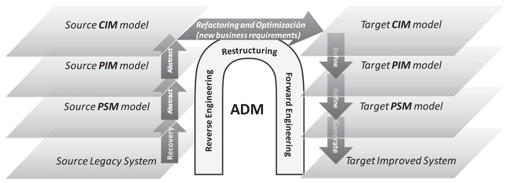
\includegraphics[width=0.49\textwidth,height=\textheight]{../figures/adm_horseshoe_1.png}\label{fig:adm-horseshoe-a}}

\subfloat[ADM standards \autocite{Perez-Castillo2011KDM}]{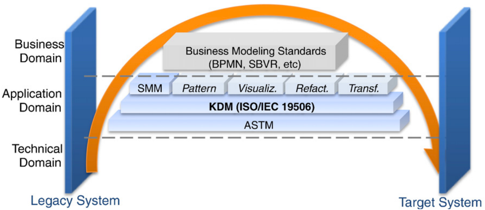
\includegraphics[width=0.49\textwidth,height=\textheight]{../figures/adm_horseshoe_2.png}\label{fig:adm-horseshoe-b}}

\caption{ADM Horseshoe}

\label{fig:adm-horseshoe}

\end{figure}

\hypertarget{tbl:adm-usage}{}
\begin{longtable}[]{@{}lllll@{}}
\caption{\label{tbl:adm-usage}Usage of ADM standards in web migration methods}\tabularnewline
\toprule
\begin{minipage}[b]{0.30\columnwidth}\raggedright
ADM\strut
\end{minipage} & \begin{minipage}[b]{0.19\columnwidth}\raggedright
KDM\strut
\end{minipage} & \begin{minipage}[b]{0.14\columnwidth}\raggedright
ASTM\strut
\end{minipage} & \begin{minipage}[b]{0.14\columnwidth}\raggedright
SMM\strut
\end{minipage} & \begin{minipage}[b]{0.10\columnwidth}\raggedright
QVT\strut
\end{minipage}\tabularnewline
\midrule
\endfirsthead
\toprule
\begin{minipage}[b]{0.30\columnwidth}\raggedright
ADM\strut
\end{minipage} & \begin{minipage}[b]{0.19\columnwidth}\raggedright
KDM\strut
\end{minipage} & \begin{minipage}[b]{0.14\columnwidth}\raggedright
ASTM\strut
\end{minipage} & \begin{minipage}[b]{0.14\columnwidth}\raggedright
SMM\strut
\end{minipage} & \begin{minipage}[b]{0.10\columnwidth}\raggedright
QVT\strut
\end{minipage}\tabularnewline
\midrule
\endhead
\begin{minipage}[t]{0.30\columnwidth}\raggedright
REMICS, PRECISO, CloudMIG, L2CMH, MIGRARIA, serviciFi\strut
\end{minipage} & \begin{minipage}[t]{0.19\columnwidth}\raggedright
ARTIST, REMICS, CloudMIG, MIGRARIA\strut
\end{minipage} & \begin{minipage}[t]{0.14\columnwidth}\raggedright
ARTIST, REMICS, MIGRARIA\strut
\end{minipage} & \begin{minipage}[t]{0.14\columnwidth}\raggedright
ARTIST, REMICS, CloudMIG\strut
\end{minipage} & \begin{minipage}[t]{0.10\columnwidth}\raggedright
PRECISO, MIGRARIA\strut
\end{minipage}\tabularnewline
\bottomrule
\end{longtable}

\hypertarget{remip}{%
\subsection{ReMiP}\label{remip}}

Sneed et al.~introduce a reference model for software migration called Reference Migration Process (ReMiP) \autocite{Sneed2010ReMiP,Gipp2007ReMiP}.
It aims at providing a general and adaptable framework for understanding and describing arbitrary software migration processes and is based on a synthesis of existing software evolution and software development methods.
A software migration is considered as a project and ReMiP's focus is on the management perspective of this project.
ReMiP structures relevant activities according to temporal and logical aspects (cf.~\cref{fig:remip}).
From the temporal perspective, activities are assigned to \emph{migration phases}.
From the logical perspective, activities are grouped into migration-specific \emph{core disciplines} and cross-cutting supporting \emph{base disciplines}.
ReMiP distinguishes four phases: \emph{Preliminary Study}, which comprises technical, economical and organisational feasibility analysis, \emph{Conceptualization and Design}, addressing migration planning activities such as legacy analysis, strategy selection and target architecture specification, \emph{Migration and Transition}, conducting iterative package-wise transformation, testing and delivery, and \emph{Closing down}, comprising activities to archive project documentation and ensure continuous operation of the migrated system.
Each phase is terminated by a milestone which serves as decision point whether to continue the migration.
These four milestones are: project objective \& process recommendation, binding master plan, migrated system release and final documentation.
The migration-specific core disciplines are \emph{requirements analysis}, \emph{legacy analysis}, \emph{target design}, \emph{strategy selection}, \emph{implementation}, \emph{test} and \emph{deployment} and represent activities from (forward) software engineering extended for migration (e.g.~requirements analysis or target design) as well as activities intrinsic to the migration domain (e.g.~legacy analysis or strategy selection).
The core disciplines are supported by base disciplines addressing cross-cutting activities to provide the operational context of the migration project.
The base disciplines are: \emph{configuration \& change management}, \emph{project management}, \emph{staff qualification} and \emph{migration environment}.
The holistic view of the ReMiP reference model provides a framework for understanding the context of software migration and thus web migration.
The definition of requirement S2 refers to the ReMiP phases.
In \cref{sec:remip-mapping} we provide mappings of the solutions provided in this thesis to ReMiP phases and disciplines.

\begin{figure}
\hypertarget{fig:remip}{%
\centering
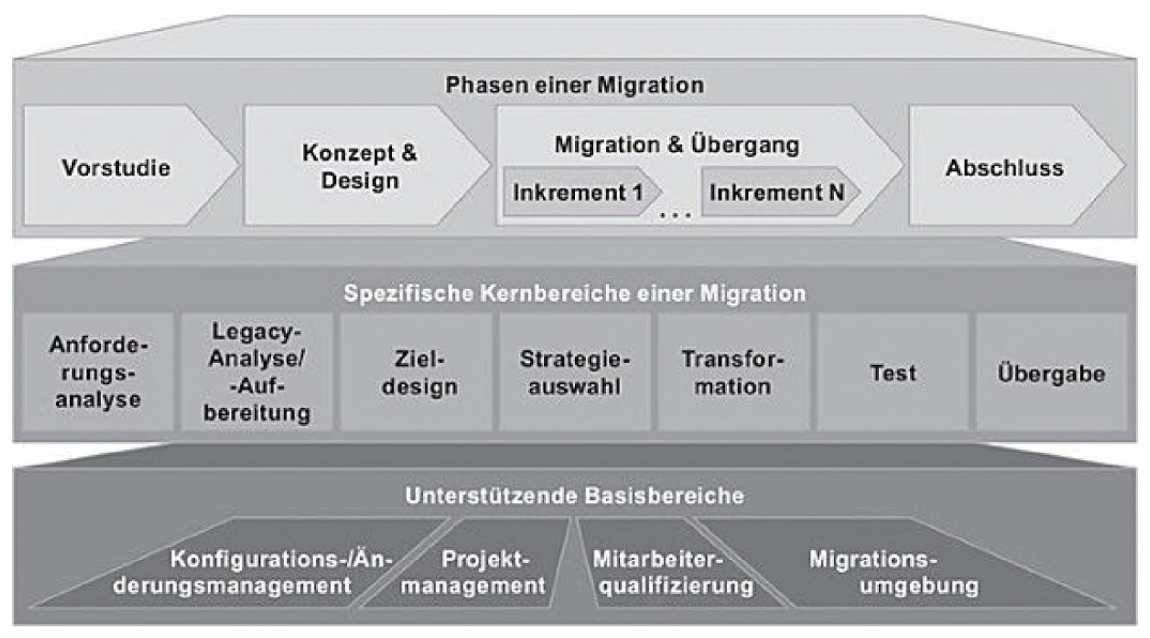
\includegraphics[width=0.99\textwidth]{../figures/remip.pdf}
\caption{ReMiP Overview \autocite[adapted from][]{Sneed2010ReMiP}}\label{fig:remip}
}
\end{figure}

\hypertarget{soa-mf}{%
\subsection{SOA-MF}\label{soa-mf}}

Razavian and Lago introduced the SOA migration framework (SOA-MF) \autocite{Razavian2013PHD,Razavian2010SOA-MF,Razavian2010,Razavian2010SurveySOAMigration} based on systematic literature review (SLR) on SOA migration techniques.
SOA migration is a research focus within the web migration field which has received significant interest (cf.~\cref{sec:soa-migration}).
SOA-MF considers migration of legacy systems to SOA as a reengineering problem, and presents an extended version of SEI's reengineering horseshoe model \autocite{Kazman1998Horseshoe}, with the three sub-processes reverse engineering, transformation and forward engineering.
In the conceptual model of SOA-MF (cf.~\cref{fig:soa-mf}), migration is considered as a transformation of \emph{artifacts} through \emph{activities} supported by \emph{knowledge}, which takes place at different \emph{levels of abstraction} between code and enterprise level.
The reverse engineering sub-process analyses and recovers the legacy architecture into higher-level abstract representations, allowing to identify migration candidates and relevant knowledge in the legacy codebase input artifact.
Transformation is conducted on representations within the same level of abstraction, altering design elements, architecture, business models and strategies.
Forward engineering renovates the selected parts of the legacy system according to new requirements into a service-based version through service implementation and service composition.
The activities of these three sub-processes are supported by code-related, design element-related, composition and business domain knowledge.
SOA-MF describes a reference model for a complete SOA migration process, existing migration methods do not necessarily employ all artifacts, activities and knowledge types.
It defines a questionnaire-based method for mapping arbitrary SOA migration approaches to SOA-MF according to coverage.
Application of this mapping on existing literature has identified eight distinct families of approaches \autocite{Razavian2013PHD,Razavian2010SurveySOAMigration}.
SOA-MF compliments ReMiP's project management focus as a reference model putting more emphasis on technical and business process aspects of migration in ReMiP phases two and three.

\begin{figure}
\hypertarget{fig:soa-mf}{%
\centering
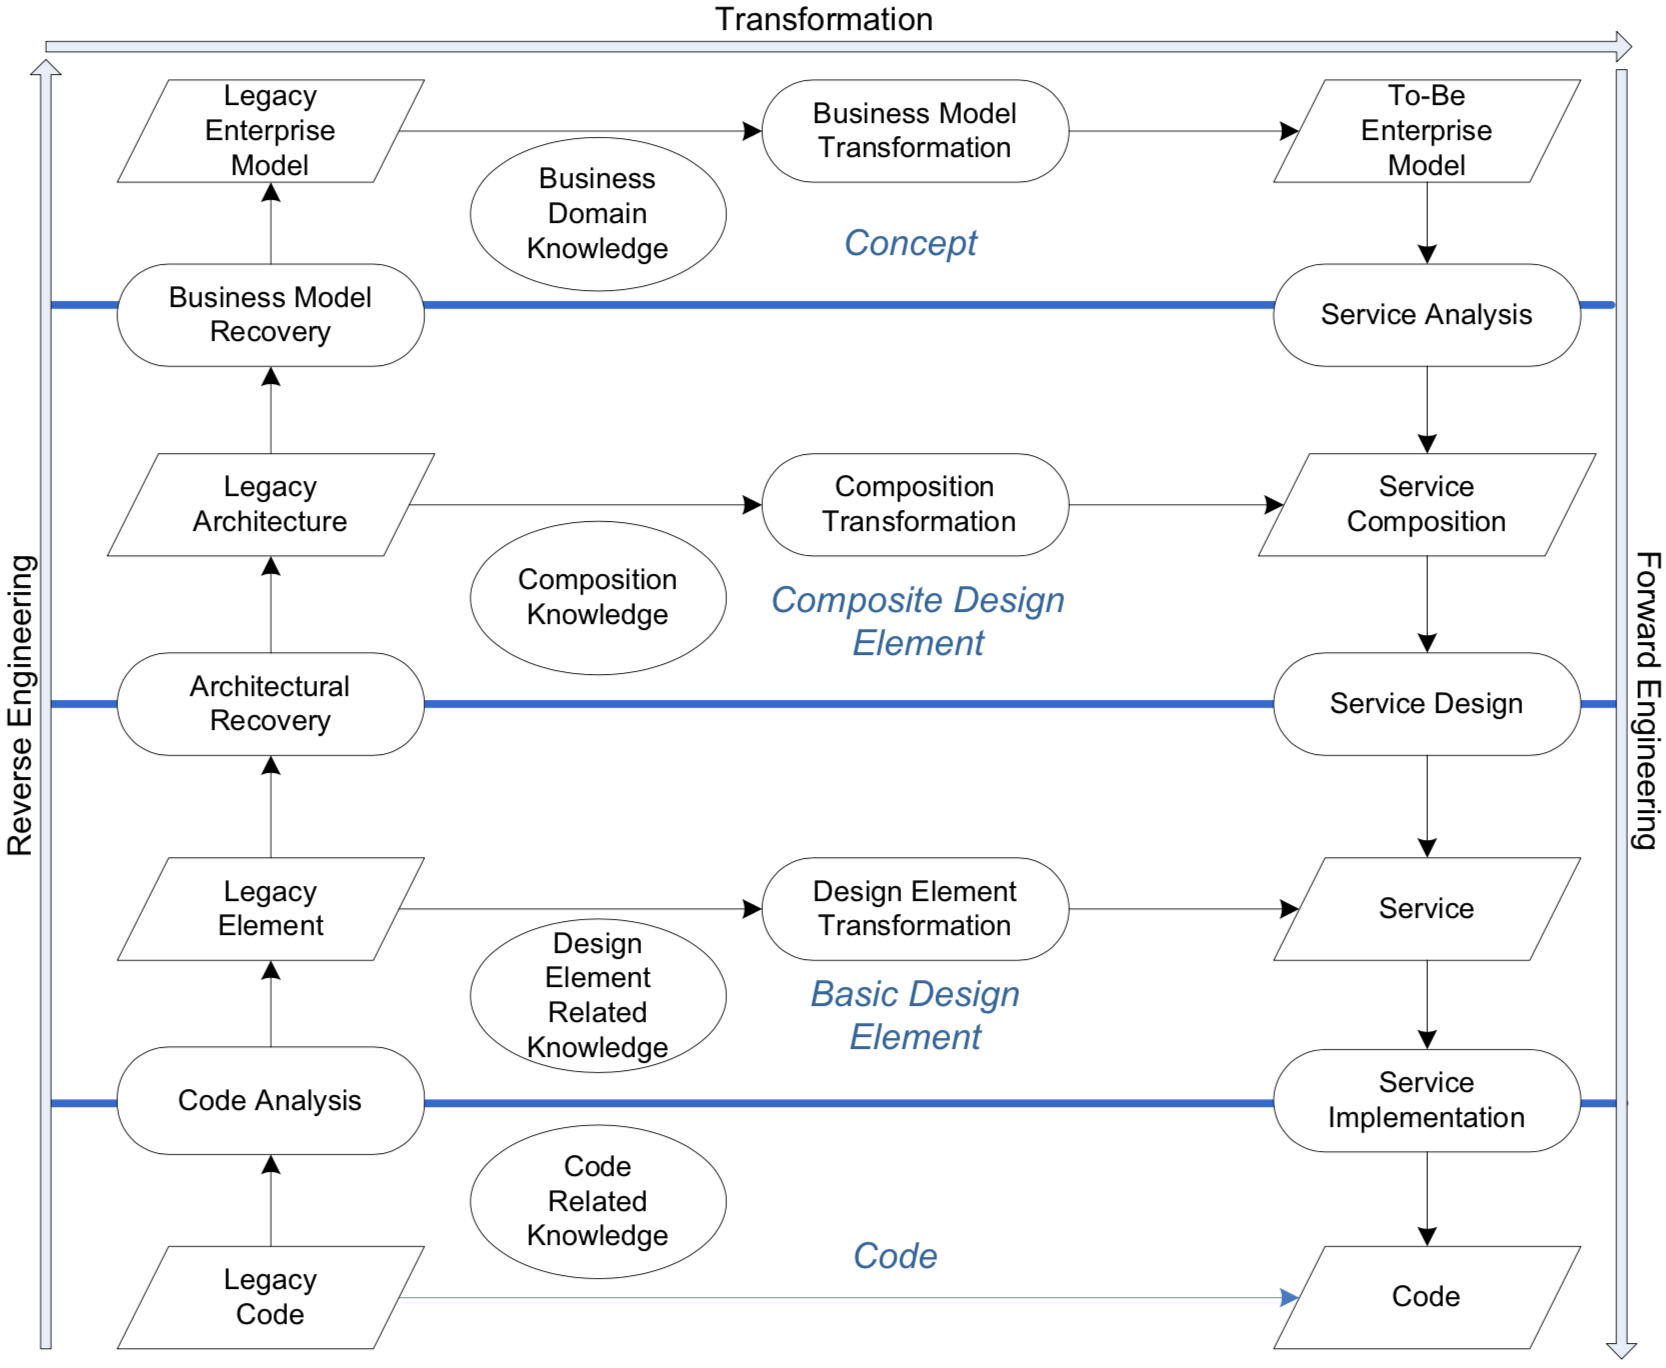
\includegraphics[width=0.99\textwidth]{../figures/soa-mf.png}
\caption{SOA-MF Overview \autocite{Razavian2010}}\label{fig:soa-mf}
}
\end{figure}

\hypertarget{sec:approaches}{%
\section{Web Migration Approaches}\label{sec:approaches}}

This section surveys the state of the art of web migration approaches.
It is organised in four groups: SOA, Cloud, Web Systems Evolution and Web Application.
These groups are defined by the target environment (SOA, Cloud, Web Application) and source system (Web Systems Evolution) and represent areas of interest in web migration research.
We identified these groups in our \emph{systematic mapping study} \autocite{Heil2017Survey} which serves as basis for this state of the art analysis.
While the scope of this previous survey was wider, comprising 122 primary studies and tools resulting from inclusion/exclusion criteria-based study selection from 870 initial search results from queries and snowballing across six data sources including dedicated methods and tools for specific migration disciplines (cf.~ReMiP), the following 22 approaches represent a condensed and updated overview on the state of the art of web migration in 2018, focusing on comprehensive approaches with high \emph{migration discipline coverage} (cf.~\autocite{Heil2017Survey}), multi-publication approaches and larger scale research projects.
The following sections will briefly introduce the four groups and report on corresponding approaches in terms of their name, related publications, research project, overall aim, main focus, method and evaluation results according to the requirements introduced in \todo{TODO:REF\_REQUIREMENTS}.

\hypertarget{sec:soa-migration}{%
\subsection{Migration to SOA}\label{sec:soa-migration}}

Service Oriented Architectures are one of the major target environments of web migration.
SOA is a business-driven approach that abstracts software by decomposition into loosely-coupled services enabling to address rapidly changing business needs through reuse of existing software assets \autocite{Gold2004SOA}.
A \emph{SOA service} is a ``coarse-grained, discoverable, and self- contained software entity that interacts with applications and other services through a loosely coupled, often asynchronous, message-based communication model'' \autocite{Lewis2005SMART}.
While SOA services exist outside the web environment, the ``most common form of SOA implementation is that of \emph{web services}'' \autocite{Lewis2008SMART}, typically with a WSDL service interface description and SOAP over HTTP communication.
Therefore, a significant share of web migration research is on SOA migration, with the goal to ``reengineer the legacy systems into a set of services which can be dynamically selected and are distributed across organization boundaries'' \autocite{Razavian2014a}.
It is worth noting that SOA migration research focuses on target systems that adhere to the fine grained SOA notion of \emph{microservices} - i.e.~one application composed of a set of small services - than on integrating several applications through services to build federated applications.
However, the term microservices was coined much later and since it is commonly used in literature, we employ the term \emph{SOA migration} to describe the entire range of migration towards web services in both the federated SOA and microservices flavor.
For more details on SOA migration refer to the dedicated surveys \autocite{Khadka2013SurveySOAMigration,Razavian2011SOASurvey,Almonaies2010SOAStrategies}.

\hypertarget{smart}{%
\subsubsection{SMART}\label{smart}}

CMU SEI's SMART method \autocite{Lewis2008SMART,Lewis2005SMART} originally published in 2005 as Service Migration and Reuse Technique is a decision-making and planning approach for the migration of legacy components to services.
SMART provides a process for legacy analysis, service identification and definition of the target SOA environment, a service migration interview guide (SMIG), a tool for automating data collection from SMIG and artifact templates for various analysis results.
The iterative SMART process starts with establishing the migration context, including analysis of business and technical context, stakeholder analysis, legacy system understanding and service identification following a top-down - based on business and mission goals and processes - and bottom-up - based on existing legacy functionality - approach resulting in a business process to service mapping.
Great emphasis is put on the migration feasibility decision, taking into account migration potential according to a set of proposed determinations.
A subset of candidate services is identified and specified in further detail, information about the legacy system is gathered in more detail through interviews with technical staff, and the target SOA environment is defined.
Gap analysis is used to provide estimates of cost, risk and effort to migrate the candidate service to the target SOA environment.
All information gathered in the previous activities feeds into the definition of the migration strategy that can include a pilot project, migration guidelines, migration path (encapsulation, transformation, reengineering) etc.
Based on experience in applying SMART, SEI realised that many organizations were not ready, did not know enough about SOA to consider migration or had not identified a particular system to migrate, so the scope of SMART was extended along with a redefinition of the acronym to SOA Migration, Adoption, and Reuse Technique \autocite{Lewis2010SMART}.
In its extended version\footnote{based on the 2013 SMART materials available at https://resources.sei.cmu.edu/library/asset-view.cfm?assetid=508038}, the original SMART method is now one of five variations of the SMART process, which form a family of related techniques addressing different organisational needs.
SMART-MP (migration pilot) represents the original perspective, SMART-AF (adoption feasibility) supports organizations' decision making whether to migrate to SOA, SMART-ESP (enterprise service portfolio) supports to select from several legacy systems which parts to expose as services, SMART-ENV (SOA environment) supports building the required SOA infrastructure and SMART-SYS (Service-Oriented Systems Development) combines all of the before mentioned variations.
SMART has influenced following migration approaches such as REMICS \autocite{REMICS2013Handbook,Mohagheghi2011REMICS}.
SMART in all variations has a desicated focus on phases prior to migration, but does not include communication of necessity and benefits of the migration.
It is designed for migration to SOA-based web systems, web-based user interfaces are not considered.
Risk management is prominently addressed, including basic techniques like feasibility assessment, incremental activities updating artifacts and incremental process as well as migration pilots.
Data about cost, risk and effort are gathered contributing to the business case and relevant knowledge is captured from the legacy system.
SMART enables reuse of functionality, but not user interaction.
Expertise requirements for SMART are not high due to the simple, well-defined process and activities and the tools and templates guiding each step.
Integration into ongoing development is not described, neither on process nor artifact level.

\hypertarget{tbl:SMART-eval}{}
\begin{longtable}[]{@{}llllll@{}}
\caption{\label{tbl:SMART-eval}SMART Evaluation}\tabularnewline
\toprule
S1 Initial & S2 Web & C1 Risk & C2 Reuse & C3 Exp & C4 Agile\tabularnewline
\midrule
\endfirsthead
\toprule
S1 Initial & S2 Web & C1 Risk & C2 Reuse & C3 Exp & C4 Agile\tabularnewline
\midrule
\endhead
\LEFTcircle & \LEFTcircle & \CIRCLE & \LEFTcircle & \CIRCLE & \Circle\tabularnewline
\bottomrule
\end{longtable}

\hypertarget{sapiensa}{%
\subsubsection{SAPIENSA}\label{sapiensa}}

SAPIENSA (Service-enAbling Pre-exIsting ENterpriSe Assets) \autocite{Razavian2010SAPIENSA,Razavian2013PHD,Razavian2012,Razavian2014a,Razavian2009} is a SOA migration research project\footnote{https://www.nwo.nl/en/research-and-results/research-projects/i/19/4019.html} under the Dutch Joint Academic and Commercial Quality Research and Development (Jacquard) program on Software Engineering in the context of which Razavian et al.~developed a SOA migration method based on knowledge management focusing on a rational investigation of legacy assets as candidate services, isolation of their properties and transformation into business services.
SAPIENSA results also contributed to EU FP7 project S-CUBE\footnote{https://cordis.europa.eu/project/reference/215483}.
The SAPIENSA method aims at exploiting architectural knowledge to enable transformation to services on different SOA abstraction levels\footnote{cf.~to abstraction levels in SOA-MF}.
Its focus on on knowledge management acknowledges importance of knowledge in migration projects.
Similar to SMART, SAPIENSA employs a \emph{middle-out} strategy, combining top-down domain and business decomposition with bottom-up legacy understanding.
The SAPIENSA process consists of three phases: architectural knowledge (AK) elicitation, transformation and service composition.
The AK elicitation extracts and externalises problem-related (e.g.~business processes and rules) and solution-related (e.g.~structure, design decisions and rationale) knowledge and identifies candidate services.
Transformation is carried out on all levels of abstraction: design elements are reshaped, architecture is restructured and business models and strategies are altered.
The service composition phase focuses on service-based forward engineering using the service composition model (SCM) leveraging services obtained from the legacy system, newly developed services and external services.
Transformation is supported by model-driven gap analysis \autocite{Nguyen2009} between as-is and to-be parts of AK such as as-is business process portfolio and to-be business process portfolio, identifying discrepancies and identifying realisation strategies.
These strategies enable decision making about re-using or re-structuring legacy assets or re-developing them and serve as input to lower-level service transformation.
The SAPIENSA approach has been elaborated in the lean and mean migration strategy \autocite{Razavian2012,Razavian2014a}, generalising core migration activities from common industry practices.
SAPIENSA adresses phases prior to migration, but does not contribute to communicate necessity and benefits.
The target system is a service-based web system, migration of GUI is not considered.
No risk management is proposed.
Reuse of legacy assets is employed to retain functionality, but user interaction is not considered.
Since the SAPIENSA process is not bound to complex transformation methods or technologies, expertise requirements are not high, but no supporting tools are provided.
Integration into ongoing development is not addressed.
SAPIENSA contributed to systematising research on SOA migration by producing the previously introduced conceptual SOA migration reference framework SOA-MF which has contributed to the understanding of migration processes and knowledge in legacy systems of this thesis as described in \todo{TODO:REF\_Knowledge\_Chapter}.

\hypertarget{tbl:SAPIENSA-eval}{}
\begin{longtable}[]{@{}llllll@{}}
\caption{\label{tbl:SAPIENSA-eval}SAPIENSA Evaluation}\tabularnewline
\toprule
S1 Initial & S2 Web & C1 Risk & C2 Reuse & C3 Exp & C4 Agile\tabularnewline
\midrule
\endfirsthead
\toprule
S1 Initial & S2 Web & C1 Risk & C2 Reuse & C3 Exp & C4 Agile\tabularnewline
\midrule
\endhead
\LEFTcircle & \LEFTcircle & \Circle & \LEFTcircle & \LEFTcircle & \Circle\tabularnewline
\bottomrule
\end{longtable}

\hypertarget{servicifi}{%
\subsubsection{ServiciFi}\label{servicifi}}

The ServiciFi method for SOA Migration presented in {[}\textcite{Khadka2011ServiciFi};Khadka2016PHD{]} is part of the ServiciFi project\footnote{https://servicifi.wordpress.com} which aims at transforming monolithic software of the financial services domain into services to enable the creation of new SOA-based applications.
As common for SOA migration approaches, it focuses on service identification, extraction and transformation.
The ServiciFi method itself was created using method engineering to assemble method fragments from three popular service-oriented development methods (SODDM, WSIM, SOMA).
It addresses phases prior to migration and includes analysis of technical feasibility and economical viability.
Portfolio analysis is used to provide a cost-benefit overview and comprises preliminary return on investment in terms of estimated maintenance cost and business value in relation to market needs.
The main part of the process is iterative.
While legacy artifacts like documentation, or UML diagrams are analysed if existing, there is no systematic recovery and re-use of legacy assets apart from what is technically needed for service extraction.
This extraction is carried out in three phases: manual service identification, specification and construction \& testing.
ServiciFi employs \emph{concept slicing}, a method that combines \emph{program slicing} with \emph{Hypothesis-Based Concept Assignment (HB-CA)} to extract an executable concept slice \autocite{Gold2005ConceptSlicing}.
However, ServiciFi does not provide tool support for this core activity, requiring manual concept slicing even in the small-scale migration case studies presented in its evaluation.
The process itself is designed as stand-alone process with no integration into existing development processes.
It is noteworthy that the situation of legacy systems in the financial services sector described as context for ServiciFi is similar to the situation described in \todo{TODO:REF\_SCENARIO}.
The ServiciFi research project has furthermore produced insightful surveys \autocite{Khadka2014ProfessionalsModernization,Batlajery2014IndustrialSurveyModernization} on legacy software and software modernization from industry practitioners' perspective which have contributed to the motivation and the problem understanding of this thesis as described in \todo{TODO:REF\_INTRO}.

\hypertarget{tbl:serviciFi-eval}{}
\begin{longtable}[]{@{}llllll@{}}
\caption{\label{tbl:serviciFi-eval}serviciFi Evaluation}\tabularnewline
\toprule
S1 Initial & S2 Web & C1 Risk & C2 Reuse & C3 Exp & C4 Agile\tabularnewline
\midrule
\endfirsthead
\toprule
S1 Initial & S2 Web & C1 Risk & C2 Reuse & C3 Exp & C4 Agile\tabularnewline
\midrule
\endhead
\LEFTcircle & \LEFTcircle & \CIRCLE & \LEFTcircle & \Circle & \Circle\tabularnewline
\bottomrule
\end{longtable}

\hypertarget{marchetto2008}{%
\subsubsection[Marchetto2008]{\texorpdfstring{Marchetto2008\footnote{this identifier was assigned to the approach due to lack of a name by the authors}}{Marchetto2008}}\label{marchetto2008}}

The approach presented by Marchetto et al.~in \autocite{Marchetto2008} aims at migrating legacy Java GUI desktop applications based on the MVC (Model-View-Controller) pattern\footnote{http://wiki.c2.com/?ModelViewController} into Web-service based versions.
It focuses on a stepwise migration process that aims at providing concrete guidance to developers and on recommending concrete existing support tools from the Java world for these steps due to the identified lack of such concrete guidance in published approaches.
The approach makes use of the UML4SOA UML profile to describe the service oriented target architecture, consisting of entity, task and utility services described through WSDL \autocite{W3C2007WSDL2.0} service descriptions.
The six-phase-process includes five phases prior to migration, but these are focused on knowledge recovery.
Migration to SOA is achieved by replacing method invocations by service invocations in the existing Java desktop GUI.
This process is incremental, successively identifying and migrating more services.
Knowledge re-discovery is limited to functionality, that is then codified in use case diagrams.
Determination of the underlying business process is indicated by the authors, but without a specified methodology or codification e.g.~as BPMN\footnote{https://www.omg.org/spec/BPMN/} diagram etc.
Due to the equality of source and target programming platform, Java, the Web Services are created by wrapping existing source code fragments in the backend.
This is achieved through a semi-automatic wrapper approach, employing the Apache Axis2\footnote{http://axis.apache.org/axis2/java/core} toolchain to create the WSDL descriptions and client stubs to invoke the services.
The GUI is left unchanged and therefore reused in its entirety, thus reuse of both functionality and user interaction are maintained.
Since the resulting application is still a Java desktop application with a web service backend, the expertise requirements are not very high.
Staff with expertise in the legacy environment can conduct the concrete step-wise process with available tool support.
Integration with ongoing development processes is not considered.

\hypertarget{tbl:Marchetto2008-eval}{}
\begin{longtable}[]{@{}llllll@{}}
\caption{\label{tbl:Marchetto2008-eval}Marchetto2008 Evaluation}\tabularnewline
\toprule
S1 Initial & S2 Web & C1 Risk & C2 Reuse & C3 Exp & C4 Agile\tabularnewline
\midrule
\endfirsthead
\toprule
S1 Initial & S2 Web & C1 Risk & C2 Reuse & C3 Exp & C4 Agile\tabularnewline
\midrule
\endhead
\Circle & \LEFTcircle & \Circle & \CIRCLE & \CIRCLE & \Circle\tabularnewline
\bottomrule
\end{longtable}

\hypertarget{soamig}{%
\subsubsection{SOAMIG}\label{soamig}}

SOAMIG \autocite{Fuhr2013SOAMIG,Winter2011SOAMIG,Zillmann2011SOAMIG} is a research project\footnote{http://www.soamig.de/ accesible through Wayback Machine snapshot from March 7, 2018: https://web.archive.org/web/20180307090643/www.soamig.de, see also https://www.offis.de/offis/projekt/soamig.html} funded by the German ministry of education and research (BMBF) under the KMU Innovativ programme which aims at the creation of a universally applicable process model for the semi-automatic migration of legacy systems into service-oriented architectures based on model-driven techniques and code transformation.
It focuses on model-driven and service identification and transformation towards Java-based web services.
The SOAMIG process \autocite{Zillmann2011SOAMIG} has four phases: preparation, conceptualization, migration and transition.
The SOAMIG migration method extends IBM's Service-Oriented Modeling and Architecture (SOMA) method \autocite{Arsanjani2008SOMA}.
It integrates SOMA's forward engineering approach with graph-based reengineering technologies.
A TGraph approach is employed to represent and analyze legacy code, supporting subsequent service identification and implementation.
SOMA is applied to specify and design services and TGraph technology-based querying and transformation techniques are applied to transfer legacy code into a service implementation.
The legacy system is parsed into TGraph models following TGraph schemas specified in grUML UML profile to describe the structure of the legacy source code and the models are stored in a graph repository together with manually modelled business processes and the target TGraph schema.
Further transformation is based on two domain-specific languages: GReQL for queries over graph repository and GReTL for transformation to target TGraph schema.
\emph{Dynamic analysis} using AspectJ traces manual execution runs of scenarios by users to identify services for the modelled business processes and is supported by the SOAMIG Business Process Tracer tool.
SOAMIG proposes two methods for service implementation: \emph{program slicing} based on results of static analysis and allocation of classes to business processes based on method invocation freuqencies based on results from dynamic analysis.
Both methods are supported by GReQL queries and help identifying service implementation code in the legacy codebase.
Results are verified by a developer and then transformed into Java code and WSDL for the web services based target implementation using GreTL and GraBaJa for code generation.
While early publications indicated application also to non-Java legacy systems, COBOL in particular, only Java is fully supported in the transformation approach two years after project end.
Phases before migration are addressed, but only focus on technical details.
The target system is a service-oriented web system, but SOAMIG does not address web-based user interfaces.
Basic risk management methods like technical feasibility study and an iterative process model are present, but the business case is no addressed, extracted knowledge is technically required for the transformation.
Reuse focuses on functionality, user interaction is no addressed.
Expertise requirements are high due to the complex model-driven methods, tools and querying and transformation languages used.
The stand-alone process does not address integration.

\hypertarget{tbl:SOAMIG-eval}{}
\begin{longtable}[]{@{}llllll@{}}
\caption{\label{tbl:SOAMIG-eval}SOAMIG Evaluation}\tabularnewline
\toprule
S1 Initial & S2 Web & C1 Risk & C2 Reuse & C3 Exp & C4 Agile\tabularnewline
\midrule
\endfirsthead
\toprule
S1 Initial & S2 Web & C1 Risk & C2 Reuse & C3 Exp & C4 Agile\tabularnewline
\midrule
\endhead
\LEFTcircle & \LEFTcircle & \LEFTcircle & \LEFTcircle & \Circle & \Circle\tabularnewline
\bottomrule
\end{longtable}

\hypertarget{gaps2ws}{%
\subsubsection{Gaps2Ws}\label{gaps2ws}}

The GUI Applications to Web Services (Gaps2Ws) approach \autocite{Grechanik2007} aims at migrating closed, monolithic third-party desktop GUI applications (GAPs) into web services to enable interoperability.
The focus lies on enabling migration to web services without source code modifications and by nonprogrammer end users.
To achieve this, Gaps2Ws repurposes accessibility technologies and combines them with a visual programming approach.
Gaps2Ws uses GUIs as APIs, using the accessibility layer of the operating system Gaps2Ws records the sequence of GUI states and user interactions as a state machine.
The visual service designer allows end users to specify web services by connecting input parameters with GUI elements by drag-and-drop and generates and deploys the Java service implementation.
Gaps2Ws is a technical GUI-based wrapper solution without process, thus phases prior to migration are not addressed.
The target system is a service-based web system without GUI.
Risk management and knowledge recovery are not addressed.
Re-use is high for legacy functionality due to the encapsulation approach.
Expertise requirements are low since the only required human interaction is simple drag-and-drop service definition supported by a visual programming tool.
Integration into ongoing development is not considered.

\hypertarget{tbl:Gaps2Ws-eval}{}
\begin{longtable}[]{@{}llllll@{}}
\caption{\label{tbl:Gaps2Ws-eval}Gaps2Ws Evaluation}\tabularnewline
\toprule
S1 Initial & S2 Web & C1 Risk & C2 Reuse & C3 Exp & C4 Agile\tabularnewline
\midrule
\endfirsthead
\toprule
S1 Initial & S2 Web & C1 Risk & C2 Reuse & C3 Exp & C4 Agile\tabularnewline
\midrule
\endhead
\Circle & \LEFTcircle & \Circle & \LEFTcircle & \CIRCLE & \Circle\tabularnewline
\bottomrule
\end{longtable}

\hypertarget{preciso}{%
\subsubsection{PRECISO}\label{preciso}}

The PRECISO SOA migration method \autocite{Perez-Castillo2013PRECISO,Perez-Castillo2009PRECISO} aims at automatic recovery and implementation of web services from legacy systems' relational databases.
It focuses on applying an ADM-based horseshoe reengineering process.

Thus, the PRECISO process addresses the three standard ADM stages: reverse engineering, restructuring, forward engineering.
A platform-specific model is reverse engineered from the legacy database schema information according to an SQL meta-model.
This PSM is transformed into a platform-independent model represented as UML2.
The PIM is transformed into a web service PSM, which is then used to generate the implementation code.
Model-driven pattern matching is employed to discover services in the database PSM.
Creation of the PIM and derivation of the final PSM is supported by QVT or manually coded transformations.
WSDL is used as meta-model for the web service PSM and the web service implementation is based on SOAP.

PRECISO is a technical SOAP-based database wrapper migration solution, no phases prior to migration are addressed.
The target system is a service-based web system without GUI.
Risk management is not addressed, knowledge recovery considers only the data model.
Re-use is low for legacy functionality and user interaction because the encapsulation approach only addresses the persistence layer, whereas application logic and user interface are not considered.
Expertise requirements are low due to the limited scope and high automation achieved in the PRECISO tool.
Integration into ongoing development is not considered.

\hypertarget{tbl:PRECISO-eval}{}
\begin{longtable}[]{@{}llllll@{}}
\caption{\label{tbl:PRECISO-eval}PRECISO Evaluation}\tabularnewline
\toprule
S1 Initial & S2 Web & C1 Risk & C2 Reuse & C3 Exp & C4 Agile\tabularnewline
\midrule
\endfirsthead
\toprule
S1 Initial & S2 Web & C1 Risk & C2 Reuse & C3 Exp & C4 Agile\tabularnewline
\midrule
\endhead
\Circle & \LEFTcircle & \Circle & \Circle & \CIRCLE & \Circle\tabularnewline
\bottomrule
\end{longtable}

\hypertarget{migration-to-cloud}{%
\subsection{Migration to Cloud}\label{migration-to-cloud}}

Cloud computing, allowing web systems to be built based on scaleable sets of rapidly provisioned, shared resources \autocite{NIST2011CloudComputing} is another major step in the web's evolution \autocite{Kienle2014EvolutionWeb}, that has resonated in web migration research \autocite{Heil2017Survey}.
In particular the SaaS paradigm has influenced the architecture of web applications and thus web migration target architectures and methods.
However, even more than SOA, cloud computing is an independent principle applying to software systems in general \autocite{Kienle2014EvolutionWeb}.
Additional requirements due to the cloud environment such as scalability \autocite{Jamshidi2013SurveyCloudMigration}, multi-tenancy wrt.
to security \autocite{Menychtas2014ARTISTJournal}, cloud resource and provider selection \autocite{Frey2011CloudMIG} and IT operations \autocite{AmazonWebServices2018Migration} are addressed in cloud migration approaches.
In the following, we consider cloud migration approaches towards web systems - mainly SaaS applications - according to requirement S2 Web.
A more detailed overview on cloud migration research can be found in dedicated surveys \autocite{Jamshidi2013SurveyCloudMigration,Pahl2013CloudSurvey,Fahmideh2018CloudSurvey}

\hypertarget{aws-migration}{%
\subsubsection{AWS Migration}\label{aws-migration}}

Amazon provides a set of resources\footnote{https://aws.amazon.com/cloud-migration/} to support companies to migrate to the cloud, specifically to Amazon Web Services (AWS).
The proposed cloud migration approach is called AWS Migration \autocite{AmazonWebServices2018Migration,AmazonWebServices2017CAF}.
It aims at enabling cloud migration for companies through a set of methods and best practices that are combined into an iterative approach.
AWS Migration focuses on the business and planning perspective of cloud migration.
The Amazon Cloud Adoption Framework (CAF) \autocite{AmazonWebServices2017CAF} is part of AWS Migration and gives recommendations how to create an actionable plan for cloud adoption in companies by assessing readiness in terms of gaps in skills and processes in business and technical perspectives: business, people, governance and platform, security, operations.
AWS Migration acknowledges the importance of organisation culture to motivate change and proposes the AWS Organizational Change Management(AWS OCM) framework.
Six different cloud migration strategies, called the 6 R's, are recommended and selection criteria explained: re-host, re-platform, re-factor/re-architect, re-purchase, retire, retain.
Guidelines to build a business case for migration that serves as data-driven rationale for initiating migration are provided, including cost and business value.
A migration readiness assessment (MRA) process produces gaps and actions address these gaps in the six CAF areas.
Discovery of existing assets in the on-premise environment is supported by discovery tools\footnote{https://aws.amazon.com/application-discovery/} and feeds into application portfolio analysis, but is very coarse-grain, addressing only the system level like servers, databases, OS versions etc.
and not knowledge in systems.
Migration planning is recommended to employ classic project management methods.
Security, Operations and Platform perspectives are briefly explained, referencing the non-migration-specific AWS whitepapers on these topics.
Prior to execution, smaller-scale migration pilots are recommended to test processes and gain experience.
The migration execution follows a cyclic six-phase process of discover, design, build, integrate, validate, cutover.
AWS migration addresses phases prior to migration in full detail, including communication aspects.
While it can be used to migrate to SaaS, the AWS migration method addresses more general cloud migration and does therefore not fulfil the target environment web requirement.
Risk management is considered in terms of feasibility assessments, portfolio analysis, migration pilots, iterative process model and building the business case.
However, knowledge discovery is too coarse-grain due to the generic nature of AWS migration.
No specific re-use of functionality or user interaction is addressed.
Expertise requirements are high as AWS Migration proposes to first create a CCoE (Cloud Center of Excellence) with staff experienced in migration and target environment.
The process further is based on dedicated cloud teams forming a migration factory\footnote{cf.~reengineering factory \autocite{Borchers1996ReengineeringFactory} idea that migration can be factory-like product line way through standardised processes and organisation} within the company, targeting large scale companies with appropriate Human Resources and support through external partners from the AWS Migration Acceleration Program\footnote{https://aws.amazon.com/migration-acceleration-program/} (AWS MAP) and AWS Professional Services\footnote{https://aws.amazon.com/professional-services/}.
Tool support, on the other hand, is extensive and bundled in the AWS Migration Hub\footnote{https://aws.amazon.com/de/migration-hub/}.
Integration into ongoing development is not addressed.

\hypertarget{tbl:AWS-Migration-eval}{}
\begin{longtable}[]{@{}llllll@{}}
\caption{\label{tbl:AWS-Migration-eval}AWS Migration Evaluation}\tabularnewline
\toprule
S1 Initial & S2 Web & C1 Risk & C2 Reuse & C3 Exp & C4 Agile\tabularnewline
\midrule
\endfirsthead
\toprule
S1 Initial & S2 Web & C1 Risk & C2 Reuse & C3 Exp & C4 Agile\tabularnewline
\midrule
\endhead
\CIRCLE & \Circle & \LEFTcircle & \Circle & \Circle & \Circle\tabularnewline
\bottomrule
\end{longtable}

\hypertarget{remics}{%
\subsubsection{REMICS}\label{remics}}

REMICS \autocite{Krasteva2013REMICSAgile,Wendland2013REMICS,REMICS2013RecoverPrinciples,REMICS2013Migrate,Remics2013RecoverToolkit,Mohagheghi2011REMICS,Sadovykh2011REMICS,Mohagheghi2010REMICS} is an EU FP7 project\footnote{http://www.remics.eu} that aims at providing a tool-supported model-driven methodology for migrating legacy applications to interoperable service cloud platforms.
Its focus is on the development of model-driven methods and tools for the migration of legacy systems to loosely coupled systems using an ADM-based bottom up approach that combines recovery of the legacy system architecture with restructuring towards SOA and deployment and verification in the cloud environment.
The REMICS modernization method adheres to the ADM horseshoe model \autocite{Perez-Castillo2011KDM,Perez-Castillo2011MARBLE,Khusidman2007}: architectural recovery feeds into transformation which is followed by forward engineering.
The recover activity identifies business processes, business rules, components, implementations and test specifications in UML and requirements in RSL \autocite{REMICS2013Migrate}.
Semi-automatic model-to-model transformations create PIM4Cloud profile SoaML deployment models which are used in forward MDA \autocite{OMG2014MDA} engineering to generate the code of the service cloud implementation using model-to-code transformations.
Model-driven test derivation through manual requirements recovery in meetings with legacy developers, refactoring of RSL requirements and test generation using UML state machines \autocite{Wendland2013REMICS}.
REMICS employs and provides a high number of model-driven technologies and tools, among them OMG Standards ADM, KDM and ASTM with extensions like RSL supported by ReDSeeDS and SoaML, UML with several profiles and BPMN supported by the Modelio modelling tool, BLU AGE for architectural recovery, Eclipse-based Focus!MBT as test modeling environment.
REMICS agile extension \autocite{Krasteva2013REMICSAgile} maps the REMICS onto a Scrum-oriented methodology: progressing in modernization sprints by modernization teams and employing meetings and artifacts from Scrum, it employs an iterative, incremental and agile model.

REMICS addresses phases prior to migration, but communication of migration necessity and benefits is not addressed.
The target architecture is an SaaS system following the Service Cloud Paradigm, a combination of cloud computing and SOA, and includes a web-based GUI.
Basic risk management is addressed in terms of feasibility evaluations and the iterative process of the REMICS agile extension.
Knowledge recovery into models is present.
Re-use of functionality is addressed in detail through the SOA migration parts of REMICS, but maintaining user interaction is not part of REMICS.
Expertise requirements are high due to the plethora of model-driven techniques and tools employed.
REMICS has been mapped into an agile process and even though not explicitly described, integration on both process and artifact level would be possible due to high overlap to Scrum process and artifacts, leading to a half rating for this requirement.

\hypertarget{tbl:REMICS-eval}{}
\begin{longtable}[]{@{}llllll@{}}
\caption{\label{tbl:REMICS-eval}REMICS Evaluation}\tabularnewline
\toprule
S1 Initial & S2 Web & C1 Risk & C2 Reuse & C3 Exp & C4 Agile\tabularnewline
\midrule
\endfirsthead
\toprule
S1 Initial & S2 Web & C1 Risk & C2 Reuse & C3 Exp & C4 Agile\tabularnewline
\midrule
\endhead
\LEFTcircle & \CIRCLE & \LEFTcircle & \LEFTcircle & \Circle & \LEFTcircle\tabularnewline
\bottomrule
\end{longtable}

\hypertarget{artist}{%
\subsubsection{ARTIST}\label{artist}}

ARTIST (Advanced software-based seRvice provisioning and migraTIon of legacy Software) \autocite{Bruneliere2015,Menychtas2014ARTISTJournal,Bruneliere2014MoDisco,Menychtas2013ARTIST,ARTIST2014Methodology,ARTIST2015ProcessFramework,ARTIST2013Taxonomy} is an EU FP7 research project\footnote{http://www.artist-project.eu/ accesible through Wayback Machine snapshot from May 4, 2018: https://web.archive.org/web/20180504233035/http://www.artist-project.eu/} that aims at providing a comprehensive, tailorable end-to-end cloud migration methodology addressing both business and technical aspects.
ARTIST focuses on the transformation and modernization of legacy software assets and businesses to facilitate automated evolution towards cloud-based SaaS.

The ARTIST migration methodology defines roles, activities, artifacts and a process model consisting of four phases: pre-migration, migration, post-migration and migration artifacts reuse \& evolution.
Pre-migration addresses technical and economic feasibility assessment, requirement analysis and migration decision making.
The model-driven technical migration phase comprises UML-based reverse engineering using MoDisco\footnote{part of the preceding European FP6 MODELPLEX project, cf.~https://www.eclipse.org/MoDisco/}, modernization based on model-to-model transformations, model annotation and partial code generation, business and process-related modernization considering legal aspects (SLAs) and business model updates.
ARTIST's post-migration phase proposes test-based verification, validation of migration goals, availability SLA checking and cloud provider certification.
An additional focus on the life cycle of the migrated application is represented in the migration artifacts reuse \& evolution phases which addresses model reuse through a repository or web-based public marketplace as well as maintenance and evolution management aspects.

ARTIST thoroughly considers phases prior to migration, including migration decision making and benefits, however, without \emph{tangible} means of communication.
The target architecture is a cloud-based SaaS system, a web-based GUI is not addressed.
Risk management is part of the methodology in terms of technical and economic feasibility assessment, business goals conformance checking and SLA compliance verification, extensive model-driven knowledge recovery is also specified.
Re-use of functionality is addressed by the model-driven transformation process, but maintaining user interaction is not part of ARTIST.
Expertise requirements are high due to the wide range of model-driven reverse engineering and transformation techniques and tools employed.
ARTIST is specified as a stand-alone migration, so integration in ongoing development processes is not considered.

\hypertarget{tbl:ARTIST-eval}{}
\begin{longtable}[]{@{}llllll@{}}
\caption{\label{tbl:ARTIST-eval}ARTIST Evaluation}\tabularnewline
\toprule
S1 Initial & S2 Web & C1 Risk & C2 Reuse & C3 Exp & C4 Agile\tabularnewline
\midrule
\endfirsthead
\toprule
S1 Initial & S2 Web & C1 Risk & C2 Reuse & C3 Exp & C4 Agile\tabularnewline
\midrule
\endhead
\CIRCLE & \LEFTcircle & \CIRCLE & \LEFTcircle & \Circle & \Circle\tabularnewline
\bottomrule
\end{longtable}

\hypertarget{cloudmig}{%
\subsubsection{CloudMIG}\label{cloudmig}}

The CloudMIG approach \autocite{Frey2010CloudMIG,Frey2011CloudMIG,Frey2011CloudMIGContraints,Frey2012CloudMIGConformance} aims at assisting reengineers in performing semi-automatic migration of enterprise software systems to scalable and resource-efficient cloud-based PaaS/IaaS environments.
It focuses on the SaaS provider perspective, balancing resource-efficiency and scalability.

The CloudMIG method reverse engineers the legacy system into an architectural representation using OMG's KDM and a utilisation model through log analysis and the Kieker\footnote{http://kieker-monitoring.net/} software monitoring tool.
The utilisation model represents resource usage and performance characteristics using OMG's Software Metrics Meta-Model (SMM)\footnote{https://www.omg.org/spec/SMM/}.
Target cloud environment selection is enabled through modeling available cloud provider IaaS and PaaS offerings.
A subsequent generation step transforms these models into the target architecture, a mapping model and a list of constraint violations.
Rule-based heuristics allow feature allocation onto the available cloud resources.
Manual adaptions prepare the models for the final model-to-code generation step.
CloudMIG Experiments highlight the shortcomings of simple cloud migration approaches for enterprise software, demonstrating that mere deployment in IaaS does not solve over- and under-provisioning of resources.
CloudMIG also models cloud environment constraints, automatically detects violations and supports to assess technical suitability before and alignment after migration, defining a cloud suitability and alignment hierarchy.
The CloudMIG method is supported by the CloudMIG Xpress tool\footnote{https://sourceforge.net/projects/cloudmigxpress/}.

CloudMIG is a cloud migration method that does not address phases prior to migration apart from knowledge recovery.
The target system is a cloud-based SaaS application which implies a web-based UI, however this is not addressed explicitly.
Risk management is not considered.
Re-use is high for legacy functionality but user interaction is not regarded.
Expertise requirements are high due to the complex MDRE and transformation techniques.
Integration into ongoing development is not considered.

\hypertarget{tbl:CloudMIG-eval}{}
\begin{longtable}[]{@{}llllll@{}}
\caption{\label{tbl:CloudMIG-eval}CloudMIG Evaluation}\tabularnewline
\toprule
S1 Initial & S2 Web & C1 Risk & C2 Reuse & C3 Exp & C4 Agile\tabularnewline
\midrule
\endfirsthead
\toprule
S1 Initial & S2 Web & C1 Risk & C2 Reuse & C3 Exp & C4 Agile\tabularnewline
\midrule
\endhead
\Circle & \CIRCLE & \Circle & \LEFTcircle & \Circle & \Circle\tabularnewline
\bottomrule
\end{longtable}

\hypertarget{ic4}{%
\subsubsection{IC4}\label{ic4}}

The IC4 (Irish Centre for Cloud Computing and Commerce) approach \autocite{Fowley2018Experimentation,Fowley2017CloudSME,Jamshidi2015,Fowley2018Licensing} aims at reengineering legacy systems to cloud-native architectures.
It focuses on the migration planning from the perspective of SME-sized ISVs with limited cloud expertise that want to transform to SaaS providers by leveraging PaaS cloud resources with focus on experimentation-oriented feasibility studies on architecture and cost concerns to drive allocation of software components to cloud resources.

IC4 proposes an incremental and pattern-based migration process with early experimentation and performance measurements.
The IC4 process consists of four stages: Consultation with ISV CEO, ISV PaaS Infrastructure Assessment and Requirements, ISV Developer and Software Development and ISV Provisioning.
Architectural reengineering from on-premise via virtualisation and PaaS to cloud-native is supported by a migration pattern catalogue \autocite{Jamshidi2015} comprising isolated architectural transformations.
Experimentation with prototypes is proposed to address technical feasibility, performance benchmarking and compare different reengineering options and related licensing models.
IC4 links different technical cloud-based application architectures with business models in terms of costs, pricing and licensing.
It uses scenario-based risk assessment methods in combination with efficiency, complexity and security metrics.

IC4 is a cloud migration planning method that addresses phases prior to migration, however the communication of necessity and benefits is not described.
Targeting PaaS-supported SaaS applications, a web-based UI is assumed although not explicitely mentioned.
Basic risk management is considered in the planning through experimentation for analysis of technical feasibility and financial viability analysis through cost model comparisons.
The partial prototyping during experimentation also contributes to the business case, providing concrete benchmarking results, however systematic recovery and management of knowledge is not addressed.
Due to the coarse-grain backend component focus, re-use is high for legacy functionality but user interaction is not regarded.
Expertise requirements are high due to the required manual reengineering and lack of tool support.
Integration into ongoing development is not considered.

\hypertarget{tbl:IC4-eval}{}
\begin{longtable}[]{@{}llllll@{}}
\caption{\label{tbl:IC4-eval}IC4 Evaluation}\tabularnewline
\toprule
S1 Initial & S2 Web & C1 Risk & C2 Reuse & C3 Exp & C4 Agile\tabularnewline
\midrule
\endfirsthead
\toprule
S1 Initial & S2 Web & C1 Risk & C2 Reuse & C3 Exp & C4 Agile\tabularnewline
\midrule
\endhead
\LEFTcircle & \CIRCLE & \LEFTcircle & \LEFTcircle & \Circle & \Circle\tabularnewline
\bottomrule
\end{longtable}

\hypertarget{ams}{%
\subsubsection{AMS}\label{ams}}

AMS (Application Migration Solution) \autocite{Meng2011} proposes migration of legacy desktop GUI applications to the cloud through GUI recognition and reconstruction technology.
It focuses on migration of legacy systems without source code.
This is realised through technology-specific GUI recognition based on memory and handle analysis for programs based on the Microsoft Component Object Model (COM)\footnote{https://docs.microsoft.com/en-us/windows/desktop/com/component-object-model--com--portal} platform.
For each window in the legacy GUI, an HTML template is generated using the NVelocity Template Engine.
The AMS Server acts as a mediator between the legacy and the web UI, translating user interaction events to synchronise UI states.
AMS achieves application-specific desktop virtualisation in the browser for multiple users using Sandboxie\footnote{https://www.sandboxie.com} as virtualisation environment to run several instances of the legacy application simultaneously.

AMS is a technical GUI-based encapsulation solution without process, thus phases prior to migration are not addressed.
The target system is a Web System with a web-based UI mirroring the legacy UI, but not a Web Application.
Risk management and knowledge recovery are not addressed.
Re-use is high for legacy functionality and user interaction due to the encapsulation approach creating and synchronising a one-to-one web representation of the legacy desktop application.
Expertise requirements are low since the technical focus of AMS does not require manual action.
Integration into ongoing development is not considered.

\hypertarget{tbl:AMS-eval}{}
\begin{longtable}[]{@{}llllll@{}}
\caption{\label{tbl:AMS-eval}AMS Evaluation}\tabularnewline
\toprule
S1 Initial & S2 Web & C1 Risk & C2 Reuse & C3 Exp & C4 Agile\tabularnewline
\midrule
\endfirsthead
\toprule
S1 Initial & S2 Web & C1 Risk & C2 Reuse & C3 Exp & C4 Agile\tabularnewline
\midrule
\endhead
\Circle & \LEFTcircle & \Circle & \CIRCLE & \CIRCLE & \Circle\tabularnewline
\bottomrule
\end{longtable}

\hypertarget{nchc}{%
\subsubsection{NCHC}\label{nchc}}

Wang et al.~\autocite{Wang2014} from Taiwan's National Center for High Performance Computing (NCHC)\footnote{http://www.nchc.org.tw/} propose a cloud migration approach for desktop applications based on Apache Guacamole\footnote{http://guacamole.apache.org/} technology.
It aims at providing cloud-based desktop virtualisation through web technologies.
The main focus is to enhance legacy desktop applications with cloud platform advantages such as collaboration, resilience and scalability without the need for specific remote desktop clients.
Instead, a platform-independent, clientless HTML5-based remote desktop virtualisation running in the browser is proposed.
Sessions are handled by a terminal proxy serving as a gateway to the virtualised terminal servers.
This virtualisation manager controls the KVM-based hypervisor through the libvirt API and handles sessions and authentication.
Guacamole is used as clientless remote desktop gateway, translating from protocols like Microsoft RDP, VNC and SSH to the Guacamole protocol, which communicates via WebSockets to the JavaScript Guacamole client that implements the HTML5-rendering in the browser.
The NCHC cloud migration is a technical virtualisation solution without process, thus phases prior to migration are not addressed.
The target system is a Web System including a web-based UI, however this UI is an identical copy of the OS desktop running the desktop application's UI and therefore does not support web functionality such as bookmarking etc.
Risk management and knowledge recovery are not addressed.
Re-use is high both for legacy functionality and user interaction due to the encapsulation approach.
Expertise requirements are low since the there is no migration process.
Integration into ongoing development is not considered.

\hypertarget{tbl:NCHC-eval}{}
\begin{longtable}[]{@{}llllll@{}}
\caption{\label{tbl:NCHC-eval}NCHC Evaluation}\tabularnewline
\toprule
S1 Initial & S2 Web & C1 Risk & C2 Reuse & C3 Exp & C4 Agile\tabularnewline
\midrule
\endfirsthead
\toprule
S1 Initial & S2 Web & C1 Risk & C2 Reuse & C3 Exp & C4 Agile\tabularnewline
\midrule
\endhead
\Circle & \LEFTcircle & \Circle & \CIRCLE & \CIRCLE & \Circle\tabularnewline
\bottomrule
\end{longtable}

\hypertarget{l2cmh}{%
\subsubsection{L2CMH}\label{l2cmh}}

The Legacy-to-Cloud Migration Horseshoe \autocite{Ahmad2014} (L2CMH) framework aims at migrating legacy systems to cloud-based architectures through software reengineering.
The focus lies on architecture-driven migration, abstracting source code level details to preserve properties of legacy systems during cloud migration, and migration planning.
Similar to REMICS, L2CMH follows a reengineering horseshoe model inspired by OMG's ADM \autocite{Perez-Castillo2011KDM,Perez-Castillo2011MARBLE,Khusidman2007} applied to cloud migration.
It preceedes the three traditional recover, transform and develop phases with a plan phase.
The migration planning comprises feasibility (effort/cost estimation) and requirements analysis, cloud provider and migration strategy selection and produces a migration plan.
L2CMH performs architecture recovery through static code analysis and graph-based architecture model abstraction.
Transformation is driven by graph transformations applying atomic change operators.
For forward engineering the transformed cloud architecture is defined in SCA\footnote{http://oasis-opencsa.org/sca} and implementation code is generated.
The plan phase of L2CMH cloud migration addresses aspects prior to migration, but does not consider communicating necessity and benefits of migration.
The target system is a cloud-based web system, however a web-based UI is not described.
Basic risk management is addressed through a feasibility study, but the migration business case is not considered beyond effort/cost.
The transformation approach has high re-use for legacy functionality, but user interaction is not considered.
Expertise requirements are high due to the graph-based modelling and transformation techniques required and lack of concrete tool support.
Integration into ongoing development is not considered.

\hypertarget{tbl:L2CMH-eval}{}
\begin{longtable}[]{@{}llllll@{}}
\caption{\label{tbl:L2CMH-eval}L2CMH Evaluation}\tabularnewline
\toprule
S1 Initial & S2 Web & C1 Risk & C2 Reuse & C3 Exp & C4 Agile\tabularnewline
\midrule
\endfirsthead
\toprule
S1 Initial & S2 Web & C1 Risk & C2 Reuse & C3 Exp & C4 Agile\tabularnewline
\midrule
\endhead
\LEFTcircle & \LEFTcircle & \LEFTcircle & \LEFTcircle & \Circle & \Circle\tabularnewline
\bottomrule
\end{longtable}

\hypertarget{web-systems-evolution}{%
\subsection{Web Systems Evolution}\label{web-systems-evolution}}

Within web migration research, web systems evolution takes a special role because not only the target system, but also the source system is a web system.
Approaches from this group address changes of existing web-based legacy systems towards other types of web systems, e.g.~from MVC to SOA, from code-based to model-driven or from static HTML to AJAX.
They are software modernization approaches that emphasize the perfective perspective more than the adaptive perspective \autocite{ISO/IEEE2006SoftwareLifeCycle} in the dimensions of architecture, design and technology evolution \autocite{Kienle2014EvolutionWeb}.
While the majority of WSE approaches focuses on technological changes and therefore has a low migration discipline coverage, the following WSE approaches are from comprehensive research projects and are comparable to other approaches from the SOA and Cloud groups.
For more details about web systems evolution research refer to \autocite{Kienle2014EvolutionWeb} and the International Symposium on Web Systems Evolution proceedings series.

\hypertarget{migraria}{%
\subsubsection{MIGRARIA}\label{migraria}}

MIGRARIA \autocite{Sosa2014MigraSOA,Sosa2013MigraSOA,Rodriguez-Echeverria2012MIGRARIA,Rodriguez-Echeverria2010MIGRARIA} is a project\footnote{http://www.eweb.unex.es/eweb/migraria/} that aims at modernization of legacy web applications to new web paradigms: Rich Internet Applications (RIA) and Service-oriented architecture (SOA).
The early works on RIA \autocite{Rodriguez-Echeverria2012MIGRARIA,Rodriguez-Echeverria2010MIGRARIA} described in this section propose the MIGRARIA method, the later works on SOA \autocite{Sosa2014MigraSOA,Sosa2013MigraSOA} propose a different method called MigraSOA and are assessed separately in the following section MigraSOA.

The MIGRARIA method aims at modernization of legacy web applications to Rich Internet Applications (RIA).
In \autocite{Rodriguez-Echeverria2010MIGRARIA}, an aspect-oriented transformation approach from WebML\footnote{the Web Modeling Language, cf.~http://webml.deib.polimi.it/ which has later been standardised by OMG as Interaction Flow Modeling Language (IFML), cf.~https://www.ifml.org} to WebML with RIA extensions \autocite{Bozzon2006WebMLforRIA,Manolescu2005,Carughi2009} is presented, \autocite{Rodriguez-Echeverria2012MIGRARIA} focuses on transformation of Java J2EE based Web Applications to RIAs based on ADM principles.
While \autocite{Rodriguez-Echeverria2010MIGRARIA} mainly focuses on client-side storing and processing and asynchronous communication, \autocite{Rodriguez-Echeverria2012MIGRARIA} formally introduces a more comprehensive list of RIA features.
Phases before migration beyond knowledge recovery are not addressed.
Both legacy and target system are full web applications including web-based GUIs.
Risk management is not addressed.
As transformation approach, the degree of reuse is high, functionality is maintained regardless whether moved to the client side or kept on the server side.
User interaction is considered as maintained, even though switching from a traditional web application to the single page paradigm has an impact.
However, this change is arguably less significant than for non-web to web migrations and regeneration of the ``look\&feel'' of the legacy WA is stated as a requirement of the MIGRARIA method.
The expertise requirements in particular for migration itself are high due to the employed technologies like KDM for describing the legacy system and the required Model-to-Model (M2M) transformations like ATL\footnote{ATLAS Transformation Language, cf.~https://www.eclipse.org/atl/} or QVT.
Integration into ongoing development processes is not addressed.
The MIGRARIA method only reports application for small, artificial examples like the Java Pet Store Demo \autocite{Rodriguez-Echeverria2012MIGRARIA}.

\hypertarget{tbl:MIGRARIA-eval}{}
\begin{longtable}[]{@{}llllll@{}}
\caption{\label{tbl:MIGRARIA-eval}MIGRARIA Evaluation}\tabularnewline
\toprule
S1 Initial & S2 Web & C1 Risk & C2 Reuse & C3 Exp & C4 Agile\tabularnewline
\midrule
\endfirsthead
\toprule
S1 Initial & S2 Web & C1 Risk & C2 Reuse & C3 Exp & C4 Agile\tabularnewline
\midrule
\endhead
\Circle & \CIRCLE & \Circle & \CIRCLE & \Circle & \Circle\tabularnewline
\bottomrule
\end{longtable}

\hypertarget{migrasoa}{%
\subsubsection{MigraSOA}\label{migrasoa}}

The MIGRARIA project aims at modernization of legacy web applications to new web paradigms.
Under the name MigraSOA, this section describes the more recent works the project \autocite{SosaSanchez2017MigraSOA,Sosa2014MigraSOA,Sosa2013MigraSOA} which focus on SOA as target web paradigm.
Like the MIGRARIA method, MigraSOA belongs to the Web Systems Evolution group and not to SOA Migration, because the source system is already a web system: it proposes a model-driven transformation of Model-View-Controller (MVC) web applications to SOA.
Java Struts is the concrete source MVC technology.
The focus is on model-driven service identification and service code generation \autocite{Sosa2013MigraSOA} and alignment of services with BPMN Models \autocite{Sosa2014MigraSOA}.
MigraSOA uses the reverse engineering step of the MIGRARIA method to extract an instance of the MIGRARIA MVC meta-model consisting of data, operations, controlflows with Modisco, services are manually identified in this model, using model-to-model transformations based on ATL rules a Simple-SoaML\footnote{https://www.omg.org/spec/SoaML} is derived, and model-to-text transformations using Acceleo\footnote{https://www.eclipse.org/acceleo/} are used to generate the WSDL, server skeleton and wrapper invocation code to be weaved into the legacy web application using AspectJ.
For the alignment of business processes with the service layer derived form the legacy web application \autocite{Sosa2014MigraSOA}, businesses processes are manually modelled using BPMN 2.0.
Additionally, a semantic dictionary describing the domain is created by experts, containing terms and related terms (synonyms, hyponyms, meronyms).
For each task in the BPMN, a Wang-Ali similarity matrix based selection of services is then performed, comparing the synonym sets of task and service.
BPMN business processes are then extended to become executable \autocite{SosaSanchez2017MigraSOA} by adding the invocation information of the aligned services using Apache Activiti\footnote{https://www.activiti.org}.
Phases before migration are not addressed beyond reverse engineering.
Being a WSE approach, both the input and the result are web applications.
Risk management is not addressed, knowledge recovery is conducted only as required for the transformations.
Functionality and user interaction are completely re-used since the original web application is only internally re-structured to SOA.
Expertise requirements are high, considering that an ISV formerly developing an non-model-based MVC web application is required to perform a model-driven migration using complex transformation technology like ATL, Acceleo to migrate into a model-driven SOA target environment.
The proposed process does not address integration into ongoing development activities.

\hypertarget{tbl:MigraSOA-eval}{}
\begin{longtable}[]{@{}llllll@{}}
\caption{\label{tbl:MigraSOA-eval}MigraSOA Evaluation}\tabularnewline
\toprule
S1 Initial & S2 Web & C1 Risk & C2 Reuse & C3 Exp & C4 Agile\tabularnewline
\midrule
\endfirsthead
\toprule
S1 Initial & S2 Web & C1 Risk & C2 Reuse & C3 Exp & C4 Agile\tabularnewline
\midrule
\endhead
\Circle & \CIRCLE & \Circle & \CIRCLE & \Circle & \Circle\tabularnewline
\bottomrule
\end{longtable}

\hypertarget{migration-to-web-applications}{%
\subsection{Migration to Web Applications}\label{migration-to-web-applications}}

This group comprises approaches that support the defining adaption of web migration - from non-web legacy systems to web systems - that do not belong to one of the two established fields of SOA or cloud migration.
Typical source systems are desktop TUI or GUI applications and mainframe systems.
Target web systems on the other hand are diverse, ranging from near-identical copies of legacy user interfaces in HTML to completely reengineered model-driven web applications.
For more information refer to \autocite{Heil2017Survey}.

\hypertarget{melis}{%
\subsubsection{MELIS}\label{melis}}

Lucia et al.~\autocite{Lucia2008,Lucia2006} present a migration strategy and tool, called MELIS \autocite{Colosimo2007ControlledExperiments}, developed in the context of an industrial technology transfer project with an SME-sized ISV.
MELIS is part of the METAMORPHOS project \autocite{Lucia2009METAMORPHOS}, that aims at facilitating reverse engineering and migration techniques and tools in industry with a focus on web-based target architectures.
The MELIS migration strategy and tool are designed for migration of monolithic multi-user COBOL legacy systems to a multi-tier web-based architecture.
Due to low decomposability, an incremental migration strategy consisting of reengineering of the UI as Web-based UI and re-structuring and wrapping of the legacy system is proposed.
The resulting target system is a Web System with a web-based UI, however, not a Web Application since the UI is only a wrapper of the legacy GUI.
The presented migration strategy addresses phases prior to actual migration, including technical assessment of the legacy system to identify the degree of \emph{decomposability}, definition of the target environment and identification of technical problems/risks related to concrete technologies and decomposability.
Advanced risk management or recovery of knowledge are not described.
Legacy functionality is re-used due to the wrapping approach, but requires manual re-structuring of the interactive COBOL programs into separate batch programs, RMI or SOAP is used to integrated resulting components when executed distributedly.
The reengineered web UI is automatically generated from the legacy GUI following the MVC pattern.
A similar look and feel of the web UI is reported as constraint by the partner company and the automatic generation process aims at producing web UIs similar to the original ones, but systematic procedure, no concrete measures or tools are provided to reach that aim.
The proposed migration strategy requires expertise in legacy technology and migration due to the necessary re-structuring of the code to be wrapped and some web expertise for the UI reengineering, in particular for the manual adaptions of the CSS files.
The process is supported by the MELIS eclipse plugin, which generates the basic web UIs and automates deployment of the wrapped components to an application server.
Integration into ongoing development is not enabled with the presented migration strategy being designed as stand-alone process.
The survey on the state of practice of software migration \autocite{Torchiano2008ItalianSurvey} conducted as part of the METAMORPHOS research project \autocite{Lucia2009METAMORPHOS} has contributed to the motivation and the problem understanding of this thesis as described in \todo{TODO:REF\_INTRO}.

\hypertarget{tbl:MELIS-eval}{}
\begin{longtable}[]{@{}llllll@{}}
\caption{\label{tbl:MELIS-eval}MELIS Evaluation}\tabularnewline
\toprule
S1 Initial & S2 Web & C1 Risk & C2 Reuse & C3 Exp & C4 Agile\tabularnewline
\midrule
\endfirsthead
\toprule
S1 Initial & S2 Web & C1 Risk & C2 Reuse & C3 Exp & C4 Agile\tabularnewline
\midrule
\endhead
\LEFTcircle & \LEFTcircle & \LEFTcircle & \CIRCLE & \Circle & \Circle\tabularnewline
\bottomrule
\end{longtable}

\hypertarget{tuimigrate}{%
\subsubsection{TUIMigrate}\label{tuimigrate}}

TUIMigrate \autocite{Karampaglis2014} proposes an approach to migrate text-based user interface (TUI) desktop applications to the web.
The main focus lies on mitigating security threats of the target system operating in the ``hostile execution environment'' of the web without manual modifications of the source code.
Karampaglis et al.~argue that moving software towards SaaS introduces security-related risks due to exposure to a large and distributed user base that may accidentally or intendedly provide harmful inputs.
The proposed method employs middleware for automatic translation of user interactions between the TUI and a web-based UI and for data sanitisation to prevent the underlying backend from receiving potentially harmful inputs.
TUIMigrate provides a tool for automatic transformation of TUIs to web-based UIs.
The TUIMigrate middleware acts as mediator, converting user interaction on the web UI into commands for the TUI and the current state of the TUI into an XML representation which is then transformed into HTML by the web frontend.
TUIMigrate is a very technology specific approach that does not address phases prior to migration.
The target system is a Web System including a web-based UI, however, this UI is a representation of a TUI.
Risk management is not addressed.
Re-use is high due to the encapsulation approach leaving legacy functionality unchanged and the automatic transformation of the TUI to a web-based UI maintaining the original user interaction.
Expertise requirements are low, as the approach is limited to the technical perspective of transforming the UI through providing a transparent middleware.
Integration into ongoing development processes is not considered.
Note that TUIMigrate combines encapsulation - for the legacy backend - with automatic transformation - for the UI, thus, we consider TUIMigrate overall as transformation approach.

\hypertarget{tbl:TUIMigrate-eval}{}
\begin{longtable}[]{@{}llllll@{}}
\caption{\label{tbl:TUIMigrate-eval}TUIMigrate Evaluation}\tabularnewline
\toprule
S1 Initial & S2 Web & C1 Risk & C2 Reuse & C3 Exp & C4 Agile\tabularnewline
\midrule
\endfirsthead
\toprule
S1 Initial & S2 Web & C1 Risk & C2 Reuse & C3 Exp & C4 Agile\tabularnewline
\midrule
\endhead
\Circle & \LEFTcircle & \Circle & \CIRCLE & \CIRCLE & \Circle\tabularnewline
\bottomrule
\end{longtable}

\hypertarget{ms-sw}{%
\subsubsection{M\&S SW}\label{ms-sw}}

As part of the Italian research project M\&S SW (Methods and Tools for the Production of the Software, Formation and Applications), Bodhuin et al.~\autocite{Bodhuin2002DesktopWebMVC,Bodhuin2003,Bodhuin2004} investigate migration of COBOL legacy systems with character-based user interfaces towards MVC web applications.
The focus lies on wrapping the legacy system and reimplementing the UI.
The proposed incremental migration strategy \autocite{Bodhuin2002DesktopWebMVC} consists of eight phases.
The first two phases deal with COBOL-specific pre-processing of the legacy source to eliminate GOTO statements.
They are followed by three reverse engineering phases which perform static analysis to identify the objects that represent fundamental concepts of the application domain, separate user interaction from application logic using program slicing techniques and abstract the data models from persistent objects.
Automatic restructuring isolates user interaction and application logic into separate COBOL programs.
The proposed toolkit creates wrappers and reimplements the GUI, wrapped objects can be optionally reimplemented later.
While the view and controller layer of MVC are generated as JSP web application, the model layer remains unchanged, supported by a gateway architecture mediating between the legacy and the new system.
The proposed GUI Reimplementer tool supports generation of basic HTML UIs through screen scraping \autocite{Merlo1995ScreenScraping} of the character-based SCREEN SECTIONs in legacy COBOL programs.
The approach was extended for non-decomposable systems using proxies for user interface and database communication instead of re-structuring to MVC in \autocite{Bodhuin2003}.
Another extension towards grid technologies focuses on distribution aspects of the components of the target MVC architecture \autocite{Bodhuin2004}.
Introducing a directory service allowing to find legacy services to the target architecture, it can be seen as an early precursor to SOA migration that would gain significant attention in research about five years later.
M\&S SW does not address phases prior to migration beyond the technical perspective of knowledge recovery.
The target system is a Web System including a web-based UI, however, this UI is a representation of a TUI.
Risk management is not addressed.
Re-use is high due to the encapsulation of legacy functionality and automatic transformation of the TUI to a web-based UI maintaining the original user interaction.
Expertise requirements are low due to the narrow technical focus and near-complete automation.
Integration into ongoing development is not considered.

\hypertarget{tbl:Mux5cux26S-SW-eval}{}
\begin{longtable}[]{@{}llllll@{}}
\caption{\label{tbl:Mux5cux26S-SW-eval}M\&S SW Evaluation}\tabularnewline
\toprule
S1 Initial & S2 Web & C1 Risk & C2 Reuse & C3 Exp & C4 Agile\tabularnewline
\midrule
\endfirsthead
\toprule
S1 Initial & S2 Web & C1 Risk & C2 Reuse & C3 Exp & C4 Agile\tabularnewline
\midrule
\endhead
\Circle & \LEFTcircle & \Circle & \CIRCLE & \CIRCLE & \Circle\tabularnewline
\bottomrule
\end{longtable}

\hypertarget{uwauwat}{%
\subsubsection{UWA/UWAT+}\label{uwauwat}}

Distante et al.~\autocite{Distante2002,Distante2004,Distante2005,Distante2006CaseStudy,Distante2006a} propose a reengineering method for the migration of data-intensive legacy applications to ubiquitous web applications.
The focus lies on definition of a methodological approach based on conceptual user centred modelling by using the Ubiquitous Web Applications (UWA) framework and its extended transaction design model UWAT+ \autocite{Distante2005}.
For brevity, we use UWA/UWAT+ as short identifier for UWA/UWAT+ based reengineering.
A particular focus is on the interplay of content navigation and process execution, which is achieved through an extended conceptual model linking business process tasks to \emph{web transactions} \autocite{Distante2004}.
The proposed reengineering method comprises three phases: requirements elicitation, reverse engineering and forward design.
It starts with stakeholder analysis and goal-based requirements elicitation.
The reverse engineering phase abstracts and formalises knowledge from the legacy system according to UWA meta-models.
Finally, the forward design performs a model-based hypermedia re-design from the functional to the navigational paradigm, consisting of information, navigation, transaction and publishing design in UWA/UWAT+.
UWA/UWAT+-based reengineering addresses phases prior to migration, but without consideration of communication aspects.
The target system is a web application including a web-based UI.
Risk management is not addressed, knowledge recovery is present.
Re-use is high both for legacy functionality and user interaction due to systematic reverse engineering of business processes and focus on similarity of user interactions.
Expertise requirements are high due to the complexity of UWA/UWAT+ methodology and meta-models and lack of dedicated tools support.
Integration into ongoing development is not considered.

\hypertarget{tbl:UWAux2fUWAT+-eval}{}
\begin{longtable}[]{@{}llllll@{}}
\caption{\label{tbl:UWAux2fUWAT+-eval}UWA/UWAT+ Evaluation}\tabularnewline
\toprule
S1 Initial & S2 Web & C1 Risk & C2 Reuse & C3 Exp & C4 Agile\tabularnewline
\midrule
\endfirsthead
\toprule
S1 Initial & S2 Web & C1 Risk & C2 Reuse & C3 Exp & C4 Agile\tabularnewline
\midrule
\endhead
\LEFTcircle & \CIRCLE & \Circle & \CIRCLE & \Circle & \Circle\tabularnewline
\bottomrule
\end{longtable}

\hypertarget{cellest}{%
\subsubsection{CelLEST}\label{cellest}}

The Canadian CEL\footnote{abbreviation for Celcorp, the main industrial sponsor} Legacy Enhancement Software Technologies (CelLEST) \autocite{Stroulia2003,Stroulia2002,Stroulia2002Book,El-Ramly2002,Stroulia1999,Kong1999} research project\footnote{http://www.cs.ualberta.ca/\textasciitilde stroulia/CELLEST} aims at the migration of legacy mainframe applications to the web.
It focuses on migration of legacy terminal user interfaces by employing reverse engineering techniques to recover functionality in terms of user tasks, capturing these in interaction models and constructing new web-based UIs.
The CelLEST method allows to reverse engineer an executable service specification based on traces of users' interactions with the legacy system.
Similar to screen scraping approaches, the parts of the legacy system are exposed (wrapped) to the new system, however, the executable model of legacy interface behaviour is derived in a semi-automatic way.
Communication between the web-based frontend and the legacy system is related via a translating proxy.
The CelLEST process proposes five steps: execution of the legacy system in an emulator to collect interaction traces, behaviour modelling using state-transition-models, task discovery through pattern analysis, task modelling through information-exchange analysis and web GUI specification based on the identified functionalities.
The creation of the state-transition model employs semi-automatic clustering of similar UI snapshots to identify compound states using a custom feature set \autocite{Stroulia1999}.
A sequential pattern-mining algorithm \autocite{El-Ramly2002} identifies task execution patterns based on recurring similar state-transition sequences, which are reviewed by an expert.
Supported by manual annotation, inputs and outputs are identified, the command language is learned and the task model is created manually.
CelLEST automatically creates an XML specification of a form-based user interface that are executed in runtime interpreters translating to XHTML or WML.
CelLEST does not addresses phases prior to migration beyond knowledge recovery.
The target system is a Web System including a web-based UI, however the UI is a representation of a TUI.
Risk management is not addressed, knowledge recovery is present in terms of interaction modeling.
Re-use is high both for legacy functionality and user interaction due to the proposed encapsulation approach and explicit modelling of user interactions.
Expertise requirements are high in spite of the simple inductive process and extensive automation tools support \autocite{Stroulia2002}, since manual task modeling and expert reviews of unsafe inferences are required.
Integration into ongoing development is not considered.

\hypertarget{tbl:CelLEST-eval}{}
\begin{longtable}[]{@{}llllll@{}}
\caption{\label{tbl:CelLEST-eval}CelLEST Evaluation}\tabularnewline
\toprule
S1 Initial & S2 Web & C1 Risk & C2 Reuse & C3 Exp & C4 Agile\tabularnewline
\midrule
\endfirsthead
\toprule
S1 Initial & S2 Web & C1 Risk & C2 Reuse & C3 Exp & C4 Agile\tabularnewline
\midrule
\endhead
\Circle & \LEFTcircle & \Circle & \CIRCLE & \Circle & \Circle\tabularnewline
\bottomrule
\end{longtable}

\hypertarget{das}{%
\subsubsection{DAS}\label{das}}

Chen et al.~\autocite{Chen2016} propose a desktop application service (DAS) framework that aims at hosting a legacy desktop application on a web server and displaying its GUI in a browser.
The focus lies on desktop virtualisation of applications instead of entire desktops through standard web protocols.
To achieve this, DAS is implemented as web server module, providing URL-based access and instantiating the desktop applications.
It functions as a mediator, forwarding user input and graphical output between browser and the applications.
DAS consists of a lifecycle manager handling instantiation and termination of desktop applications and a set of desktop UI-library-specific service agents that handle the input/output conversions.
A service agent based on Broadway is proposed which enables translation between GTK+ and HTML5.
DAS is a technical virtualisation solution without process, thus phases prior to migration are not addressed.
The target system is a Web System including a web-based UI, however this UI is an identical representation of the virtualized desktop UI and therefore does not support web functionality such as bookmarking etc.
Risk management and knowledge recovery are not addressed.
Re-use is high both for legacy functionality and user interaction due to the encapsulation approach.
Expertise requirements are low since the there is no migration process.
Integration into ongoing development is not considered.

\hypertarget{tbl:DAS-eval}{}
\begin{longtable}[]{@{}llllll@{}}
\caption{\label{tbl:DAS-eval}DAS Evaluation}\tabularnewline
\toprule
S1 Initial & S2 Web & C1 Risk & C2 Reuse & C3 Exp & C4 Agile\tabularnewline
\midrule
\endfirsthead
\toprule
S1 Initial & S2 Web & C1 Risk & C2 Reuse & C3 Exp & C4 Agile\tabularnewline
\midrule
\endhead
\Circle & \LEFTcircle & \Circle & \CIRCLE & \CIRCLE & \Circle\tabularnewline
\bottomrule
\end{longtable}

\hypertarget{approach-classification}{%
\section{Approach Classification}\label{approach-classification}}

The approaches introduced and assessed above have been assigned into groups according to research areas and target architectures, which represents the historical development of migration research and the classification commonly used in literature \autocite{Kienle2014EvolutionWeb}.
While some commonalities with regard to the requirements can be identified among the members of these groups, the migration approaches also show unique characteristics that cannot be captured on a per-group basis.
Often tailored to a specific context, a high number of parameters determine a specific migration approach (e.g.~Migration Type, Migration Discipline, Legacy Environment, Target Environment) \autocite{Heil2017Survey}.
These form independent dimensions of description of migration approaches, which are orthogonal to the groups introduced above.
In particular, in our Survey \autocite{Heil2017Survey}, we observed that migration approaches are further divided depending on the overall methodology which they use.
We identified three main groups:

\begin{itemize}
\tightlist
\item
  \textbf{Encapsulation} approaches, that wrap the unchanged legacy system or parts of it and expose a new interface which is then integrated with the target system \autocite[cf.~to \emph{external interface}, \emph{internal implementation} in \emph{encapsulation} definition][]{ISO/IEEE24765Vocabulary},
\item
  \textbf{Reengineering} approaches, that employ \emph{reverse engineering} techniques to extract information from the legacy system and follow up with \emph{forward engineering} to create the target system (cf.~also to ISO/IEEE reengineering definition in \autocite{ISO/IEEE24765Vocabulary,IEEE1219Maintenance}) and
\item
  \textbf{Transformation} approaches, that process the legacy source code by a series of \emph{automatic transformations} turning it into the target system's source code.
\end{itemize}

Table \cref{tbl:sota-groups} provides an overview of the approaches in the two grouping schemes \emph{research areas and target architectures} and \emph{methodologies}.

\hypertarget{tbl:sota-groups}{}
\begin{longtable}[]{@{}lllll@{}}
\caption{\label{tbl:sota-groups}Overview of web migration methods wrt.
research areas/target architectures and methodologies}\tabularnewline
\toprule
& \textbf{Encapsulation} & \textbf{Reengineering} & \textbf{Transformation} & \textbf{Other}\tabularnewline
\midrule
\endfirsthead
\toprule
& \textbf{Encapsulation} & \textbf{Reengineering} & \textbf{Transformation} & \textbf{Other}\tabularnewline
\midrule
\endhead
\textbf{SOA} & Marchetto2008, Gaps2Ws, PRECISO & serviciFi & SOAMIG, SAPIENSA & SMART\footnote{addresses only phases before migration}\tabularnewline
\textbf{Cloud} & AMS, NCHC & IC4 & REMICS, L2CMH, ARTIST, CloudMIG & AWS Migration\footnote{migration planning framework without concrete encapsulation/reengineering/transformation methodology}\tabularnewline
\textbf{WSE} & & & MIGRARIA, MigraSOA &\tabularnewline
\textbf{Web Application} & MELIS, M\&S SW, CelLEST, DAS & UWA/UWAT+ & TUIMigrate &\tabularnewline
\bottomrule
\end{longtable}

A more comprehensive overview on Reengineering technologies can be found in \autocite{Perez-Castillo2011Reengineering}.
To discuss the results of the assessment of approaches in \todo{TODO:REF\_PREVIOUS\_SECTION}, findings will be reported based on research areas and target architectures, on methodologies and on individual approaches.

\hypertarget{sec:sota.discussion}{%
\section{Discussion}\label{sec:sota.discussion}}

\begin{itemize}
\tightlist
\item
  \todo{TODO: introduce explicit shortcomings S}1, S2, S3 etc.
like in \autocite{Frey2010CloudMIG}
\end{itemize}

Since software migration approaches are typically tailored to a specific environment \autocite[cf.~brownfield software engineering][]{Hopkins2008Brownfield}, the web migration approaches have been assessed each on its own above.
The two orthogonal dimensions - target architecture and methods \autocite{Heil2017Survey} - both imply common characteristics.
Therefore, this section aggregates the analysis results from the web migration approaches evaluated above and discusses commonalities in both dimensions as well as observations about the entire state of the art.

\newpage

\hypertarget{tbl:eval-overview}{}
\begin{longtable}[]{@{}llllll@{}}
\caption{\label{tbl:eval-overview}Evaluation Overview}\tabularnewline
\toprule
Approach & Target & Method & S1 Initial & S2 Web & C1 Risk\tabularnewline
\midrule
\endfirsthead
\toprule
Approach & Target & Method & S1 Initial & S2 Web & C1 Risk\tabularnewline
\midrule
\endhead
SMART & SOA & N/A & \LEFTcircle & \LEFTcircle & \CIRCLE\tabularnewline
SAPIENSA & SOA & Trans & \LEFTcircle & \LEFTcircle & \Circle\tabularnewline
serviciFi & SOA & ReEng & \LEFTcircle & \LEFTcircle & \CIRCLE\tabularnewline
Marchetto2008 & SOA & Encaps & \Circle & \LEFTcircle & \Circle\tabularnewline
SOAMIG & SOA & Trans & \LEFTcircle & \LEFTcircle & \LEFTcircle\tabularnewline
Gaps2Ws & SOA & Encaps & \Circle & \LEFTcircle & \Circle\tabularnewline
PRECISO & SOA & Encaps & \Circle & \LEFTcircle & \Circle\tabularnewline
AWS Migration & Cloud & N/A & \CIRCLE & \Circle & \LEFTcircle\tabularnewline
REMICS & Cloud & Trans & \LEFTcircle & \CIRCLE & \LEFTcircle\tabularnewline
ARTIST & Cloud & Trans & \CIRCLE & \LEFTcircle & \CIRCLE\tabularnewline
CloudMIG & Cloud & Trans & \Circle & \CIRCLE & \Circle\tabularnewline
IC4 & Cloud & ReEng & \LEFTcircle & \CIRCLE & \LEFTcircle\tabularnewline
AMS & Cloud & Encaps & \Circle & \LEFTcircle & \Circle\tabularnewline
NCHC & Cloud & Encaps & \Circle & \LEFTcircle & \Circle\tabularnewline
L2CMH & Cloud & Trans & \LEFTcircle & \LEFTcircle & \LEFTcircle\tabularnewline
MIGRARIA & WSE & Trans & \Circle & \CIRCLE & \Circle\tabularnewline
MigraSOA & WSE & Trans & \Circle & \CIRCLE & \Circle\tabularnewline
MELIS & Web & Encaps & \LEFTcircle & \LEFTcircle & \LEFTcircle\tabularnewline
TUIMigrate & Web & Trans & \Circle & \LEFTcircle & \Circle\tabularnewline
M\&S SW & Web & Encaps & \Circle & \LEFTcircle & \Circle\tabularnewline
UWA/UWAT+ & Web & ReEng & \LEFTcircle & \CIRCLE & \Circle\tabularnewline
CelLEST & Web & Encaps & \Circle & \LEFTcircle & \Circle\tabularnewline
DAS & Web & Encaps & \Circle & \LEFTcircle & \Circle\tabularnewline
\bottomrule
\end{longtable}

\hypertarget{tbl:eval-overview-methods}{}
\begin{longtable}[]{@{}llllll@{}}
\caption{\label{tbl:eval-overview-methods}Evaluation Overview by Method}\tabularnewline
\toprule
Approach & Target & Method & S1 Initial & S2 Web & C1 Risk\tabularnewline
\midrule
\endfirsthead
\toprule
Approach & Target & Method & S1 Initial & S2 Web & C1 Risk\tabularnewline
\midrule
\endhead
Marchetto2008 & SOA & Encaps & \Circle & \LEFTcircle & \Circle\tabularnewline
Gaps2Ws & SOA & Encaps & \Circle & \LEFTcircle & \Circle\tabularnewline
PRECISO & SOA & Encaps & \Circle & \LEFTcircle & \Circle\tabularnewline
AMS & Cloud & Encaps & \Circle & \LEFTcircle & \Circle\tabularnewline
NCHC & Cloud & Encaps & \Circle & \LEFTcircle & \Circle\tabularnewline
MELIS & Web & Encaps & \LEFTcircle & \LEFTcircle & \LEFTcircle\tabularnewline
M\&S SW & Web & Encaps & \Circle & \LEFTcircle & \Circle\tabularnewline
CelLEST & Web & Encaps & \Circle & \LEFTcircle & \Circle\tabularnewline
DAS & Web & Encaps & \Circle & \LEFTcircle & \Circle\tabularnewline
SMART & SOA & N/A & \LEFTcircle & \LEFTcircle & \CIRCLE\tabularnewline
AWS Migration & Cloud & N/A & \CIRCLE & \Circle & \LEFTcircle\tabularnewline
serviciFi & SOA & ReEng & \LEFTcircle & \LEFTcircle & \CIRCLE\tabularnewline
IC4 & Cloud & ReEng & \LEFTcircle & \CIRCLE & \LEFTcircle\tabularnewline
UWA/UWAT+ & Web & ReEng & \LEFTcircle & \CIRCLE & \Circle\tabularnewline
SAPIENSA & SOA & Trans & \LEFTcircle & \LEFTcircle & \Circle\tabularnewline
SOAMIG & SOA & Trans & \LEFTcircle & \LEFTcircle & \LEFTcircle\tabularnewline
REMICS & Cloud & Trans & \LEFTcircle & \CIRCLE & \LEFTcircle\tabularnewline
ARTIST & Cloud & Trans & \CIRCLE & \LEFTcircle & \CIRCLE\tabularnewline
CloudMIG & Cloud & Trans & \Circle & \CIRCLE & \Circle\tabularnewline
L2CMH & Cloud & Trans & \LEFTcircle & \LEFTcircle & \LEFTcircle\tabularnewline
MIGRARIA & WSE & Trans & \Circle & \CIRCLE & \Circle\tabularnewline
MigraSOA & WSE & Trans & \Circle & \CIRCLE & \Circle\tabularnewline
TUIMigrate & Web & Trans & \Circle & \LEFTcircle & \Circle\tabularnewline
\bottomrule
\end{longtable}

\textbf{SOA} The analysed SOA migration approaches stress the importance of identifying the functionalities (i.e.~services) of a legacy web system.
They are concerned with capturing functionality in technology-independent models and identifying the business processes which define and make use of it.
The legacy web system can be considered a \emph{service repository} \autocite{Sosa2014MigraSOA}.
Exposing legacy code as services through the two dominant methods of encapsulation or transformation requires good separation of \emph{UI code} from \emph{business or mission function code} \autocite{Lewis2008SMART}, otherwise replacement is more cost-effective.
SOA as target architectural style focuses more on re-use of exposed functionality across several systems in a larger enterprise software environment than on re-use of functionality of single systems \autocite{Lewis2008SMART}.
The emphasis on backend functionality leads to dominantly medium ratings for S2 Web and C2 Reuse.
Reverse engineering is neglected in industry for SOA migration \autocite{Razavian2012}.
The consideration of business aspects results in higher use of risk management mechanisms (C1 Risk) compared to Cloud, WSE and Web employing feasibility studies, portfolio analysis and pilots.

\textbf{Cloud} Cloud migration approaches show the highest support of phases prior to migration (S1 Initial) of all groups due to cloud-related additional planning activities such as resource allocation and decision making.
However only two approaches address business case support through communication of benefits.
The Cloud group also comprises the most comprehensive migration methodologies including the results of two EU FP7 projects.
However, cloud migration research is often focused on migrating on-premise software of large companies; the ISV perspective is seldomly represented \autocite{Fowley2017CloudSME}.
Compared to SOA's exclusive backend focus, Cloud migration approaches reach higher ratings for S2 Web due to consideration of UI aspects in some approaches that are not limited to desktop-virtualization variants.
Risk management (C1 Risk) is addressed slightly more than in SOA migration and expertise requirements (C3 Exp) are higher.
With REMICS agile extensions, the Cloud group contains the only approach addressing integration into ongoing development (C4 Agile) to some degree.

\textbf{WSE} The Web Systems Evolution approaches unanimously excel in S2 Web and C2 Reuse and fail in all other requirements.
Since the source environment is already a Web System that is modernised into a newer web-based target architecture, WSE approaches achieve full rating for the target environment.
Likewise, their transformation approaches make complete re-use of existing assets to maintain both functionality and interaction.

\textbf{Web Application} A poor support of phases before migration (S1 Initial) was observed in the mainly technical Web Application migration approaches analysed.
Similarly, due to their technical focus risk management (C3 Risk) is not present.
They rate second highest with regard to target environment (S2 Web), however not as high as expected due to the resulting web applications often being identical representations of desktop applications instead of web applications with real web UIs.
In terms of reuse of existing assets (C2 Reuse) they rate outstandingly high as the objective of these technical approaches is to transfer functionality and interaction into a web-based environment.
Mainly originating from mid-2000s and with text-based source legacy systems, the migrated target systems have to be considered outdated in terms of technology (e.g.~RMI) and user interaction (e.g.~textual console).
A certain neglect of the foundational web application migration field in favour of SOA and Cloud is evident (cf.~also \autocite{Heil2017Survey}).

\textbf{Encapsulation} Many web migration approaches are using wrapping approaches that create a hybrid legacy system that do not mitigate legacy risks, since the fundamental characteristics of the legacy system are not changed \autocite{Almonaies2010SOAStrategies} and they lead to \emph{architectural degradation}, where the ``new system delivers lower quality than pre-existing system'' \autocite{Razavian2010SAPIENSA}, and the legacy system must still be maintained in addition to the wrappers \autocite{Fuhr2013SOAMIG}, typically increasing the technological heterogeneity.
They propose a \emph{web migration without modernization} and are therefore limited to the adaptive perspective, failing to address the required perfective dimension of web migration \autocite{ISO/IEEE2006SoftwareLifeCycle}.
The resulting web-enabled legacy system does not fully achieve the web application target requirement S2 Web.
Wrapping is only applicable if legacy functionality should remain completely unchanged, otherwise program understanding and restructuring is required \autocite{Stroulia2002}.
Thus, encapsulation approaches reach the highest levels of re-use of existing assets (C2 Reuse).
As Encapsulation approaches often see migration from a system integration perspective, employing solution patterns from EAI (Enterprise Application Integration) like gateways, proxies \autocite{Karampaglis2014,Bodhuin2003}, decomposability is the pre-requisite \autocite{Wagner2014Fundamentals,Khadka2016PHD,Khadka2013SurveySOAMigration,Lucia2008,Lucia2006}.
Technical wrapper solutions like DAS, Gaps2Ws, AMS are very similar and limited to a kind of application-specific desktop virtualization in the browser.
Thus, initial phases (S1 Initial) and risk management (C3 Risk) are nearly not addressed.
Due to the simplicity, however, expertise requirements (C3 Exp) are low.

\textbf{Transformation} Transformation-based web migration approaches have a high level of re-use for functionality, but user interaction is mostly not regarded (C2 Reuse).
The automatic transformations are very platform-specific and therefore have only limited applicability.
The majority of transformation approaches follow the model-driven paradigm, extending the objective of reuse to the transformations themselves, which implies high expertise requirements (C3 Exp) due to the complex model-driven technologies used.
Due to their technical focus, support for initial phases (S1 Initial) and risk management (C3 Risk) is not widely observed in this group.
Similar to encapsulation approaches, decomposability is crucial \autocite{Khadka2016PHD,Khadka2013SurveySOAMigration,Lucia2008,Lucia2006}.
Transformation often requires additional prior re-engineering / re-structuring \autocite{Nasr2010}.

\textbf{Reengineering} Both encapsulation and transformation approaches for legacy systems with low decomposability require re-structuring \autocite{Nasr2010,Aversano2001,Wagner2014Fundamentals,Khadka2016PHD,Khadka2013SurveySOAMigration,Lucia2008,Lucia2006}.
Their advantages in terms of reduced effort are quickly mitigated, so that Reengineering becomes more viable.
Reengineering approaches have the highest support for phases prior to migration (S1 Initial) and re-use of legacy assets is high (C2 Reuse) due to their objective of changing a legacy system on different levels of abstraction that requires thorough planning and system understanding through implied reverse engineering.
However, the complex architectural changes also demand high expertise and involve a significant amount of manual activities (C3 Exp).

Independent of the groups and methods, the following section describes general characteristics and observations in the state of the art of web migration.

The vast majority of approaches follow an incremental and ``\emph{feature-driven iterative migration}'' \autocite{Menychtas2014ARTISTJournal} process model.

\textbf{Initial Phases} The majority of web migration approaches do not address the initial phases (cf.~also \autocite{Heil2017Survey}).
Among those which do so, the focus is on the economic viability perspective {[}\textcite{Khadka2011ServiciFi};Khadka2016PHD{]} in term of costs/risks/constraints \autocite{Razavian2012}.
Communication of migration benefits is widely overseen.
Even comprehensive methodologies like ARTIST and AWS Migration - which comprise general consideration of benefits through analysis of customer needs using interviews, surveys etc.
- do not propose methods to provide concrete, tangible means of communicating migration benefits to support analysis of customer and ISV benefits prior to migration decision making.

\textbf{Risk Management} Similarly risk management practices have not been observed frequently with only SMART and ARTIST comprising strategies that contribute to the business case and secure existing knowledge against loss during migration.
IC4 has a dedicated focus on risk assessment through experimentation-oriented feasibility studies.
Other approaches either do not address risk or are restricted to technical feasibility analysis.
In contrast to academia, industrial practice often relies on interviewing stakeholders for knowledge elicitation such as locating functionality in legacy code while neglecting reverse engineering \autocite{Razavian2013PHD,Razavian2012}.
However, stakeholders of long-running legacy systems as in \todo{TODO:REF\_SCENARIO are no longer available}, so the legacy source is often ``the only source of domain knowledge'' \autocite{Bodhuin2002DesktopWebMVC}.

\textbf{Re-use} While re-use of legacy artifacts for maintaining functionality is high, user interaction is disregarded.
This lack of consideration of impact on existing users is in contrast with the importance of a ``similar look and feel'' for industry \autocite{Rodriguez-Echeverria2012MIGRARIA,Lucia2008,Distante2002}.
There are no concrete metrics or tools to support achieving this objective.
Dedicated migration approaches for user interfaces are mainly focused on either character-based TUIs to the web (M\&S SW, TUIMigrate), where a nearly literal translation is simple and successful, or on browser-based desktop virtualization wrappers (DAS, Gaps2Ws, AMS), both of which create results with limited suitability for the web \autocite{Distante2006a}.

\textbf{Low Abstraction} Many approaches (eg.
MELIS, SoaMIG, M\&S SW, Marchetto2008) operate at a low abstraction level close to code (cf.~levels of abstraction in ADM and SOA-MF) , ``hindering reusability and maintainability of the obtained system'' \autocite{Sosa2014MigraSOA} and focus on technical aspects of encapsulation and transformation.
On the other hand, sophisticated methods like ARTIST, REMICS, UWA/UWAT+ consider business, organisational and architectural abstractions but have high expertise requirements.

\textbf{MD} Half of the surveyed approaches, in particular transformation approaches, are based on the model-driven paradigm, i.e.~they provide formal definitions for metamodels and transformation languages for instances of these metamodels \autocite{Fuhr2013SOAMIG}.
They employ model-driven technologies from OMG or EMP (Eclipse Modeling Project\footnote{https://www.eclipse.org/modeling/}): the proposed metamodels are mainly UML profiles and MOF compliant (OMG) or KM3 compliant (EMP), transformation languages such as QVT (OMG) and ATL (EMP) are common.
Especially OMG's ADM family languages are widely used among model-driven migration approaches as indicated in \cref{tbl:adm-usage}.
Most model-driven methodologies (e.g.~ARTIST, REMICS, SoaMIG, MELIS) are focused on the Java platform for source and target system and are built around Eclipse modeling tools like MoDisco \autocite{Perez-Castillo2011Reengineering}.
The model-driven objective of achieving re-use of not only design artifacts but also the model transformations introduces a high level of complexity which results in high expertise requirements (C3 Exp) for both the migration and the target environment.
In particular, it is assumed that the target system will be evolved in a model-driven way, which requires a fundamental change for companies previously not employing model-driven development.

\textbf{SME-sized ISVs} The finding of our 2017 systematic mapping study \autocite{Heil2017Survey}, that the perspective of ISVs, in particular small and medium-sized ISVs, is hardly considered, still holds.
IC4 does so explicitly, but due to lack of concrete reengineering methodology and tool support places high expertise requirements, lacks communication of migration benefits, systematic knowledge recovery and re-use of interaction-related assets.
Many approaches are only demonstrated with small, artificial sample applications (e.g.~conference management \autocite{Sosa2014MigraSOA}, Java Pet Store Demo \autocite{Rodriguez-Echeverria2012MIGRARIA}) that do not represent all legacy characteristics, mainly representing legacy technology but lacking size, structural degradation and technical debt.
Likewise, characteristics of SME-sized SMEs (cf.~\cref{sec:company-characteristics}) are neglected.
Feasibility of the approaches with existing staff lacking expertise in target technology and software migration (C3 Exp) is only observed for encapsulation approaches and transformation for TUIs, that have severe drawbacks as described above.
The most promising comprehensive approaches in terms of overall rating (e.g.~REMICS, ARTIST, UWA/UWAT+) all have high expertise requirements.
Integration into ongoing, agile development activities is widely overseen with all approaches designed as stand-alone processes.
Only REMICS agile extensions - although not explicitly described - could be integrated.

\textbf{Integration} Agile integration was only observed in one approach, REMICS.
In REMICS, however, it is not directly described.
Its agile extensions specify a mapping onto Scrum, which facilitates integration with an ongoing agile development process and environment.
The same characteristics are found in reengineering outside the web migration field, with approaches like PARFAIT \autocite{Cagnin2003} defining stand-alone agile reengineering processes, in this case from procedural to object-oriented business resource management systems.
Integration aspects for the most labour-expensive category of reengineering are not addressed in research.
Due to the differences in the nature of any software modernization or migration in comparison to forward engineering, integration is hard to achieve.
However, even partial integration would benefit the applicability for ISVs with limited resources.

\textbf{Methodologies}.
Comprehensive approaches like ARTIST, SAPIENSA, REMICS, and UWA/UWAT+ with full coverage according to ReMiP and popular approaches like SMART are specified as \emph{methodologies}: they provide a set of principles, formalisms, methods and tools \autocite{Wallmueller2001SoftwareQuality} for web migration.
This structure provides an implicit mechanism for extension through integration with other methodologies.
For instance, REMICS focuses on recovery, migration and deployment.
To address initial phases of web migration, it integrates methods from the SMART methodology.

The shortcomings in the current state of the art in web migration identified above make it difficult for SME-sized ISVs with legacy, non-web, desktop applications and large existing user bases to commence a web migration.
Existing approaches do not sufficiently address their doubts about feasibility and desirability that make them hesitant to take the risks of a migration project, in particular in initial phases prior to migration.
Reuse is mainly considered for backend functionality, continuity of the user interface and user interaction is neglected.
There is much focus on SOA and Cloud, migration to web applications independent of these two paradigms are not frequently considered besides simple encapsulation approaches.
Web migration approaches are evenly split between model-driven and non-model-driven approaches.
The characteristics of SME-sized ISVs are ignored by most approaches, defining complex stand-alone processes that require resources and expertise beyond availability.
Integration aspects are overseen in research.
To conclude, there are many partial solutions in the web migration field, but, in particular comprehensive methodologies like ARTIST, REMICS, UWA/UWAT+ exhibit shortcomings in important requirements and would benefit from a dedicated solution addressing these gaps.

\hypertarget{summary}{%
\section{Summary}\label{summary}}

This chapter presented relevant standards and reference models and assessed existing web migration approaches according to the requirements elicited in \cref{sec:requirements-analysis}.
A two-dimensional classification scheme was introduced and a detailed discussion of observations was presented.
This analysis has revealed the lack of a suitable solution combining support of initial phases and web application target architecture with suitability for SME-sized ISVs in terms of risk management, reuse of functionality and user interaction, available expertise and resources, and integration into ongoing agile development, demonstrating the relevancy and need for the solution presented in the following chapter.
The detailed findings have provided input for the creation of the solution concept.
